% mnras_template.tex 
%
% LaTeX template for creating an MNRAS paper
%
% v3.0 released 14 May 2015
% (version numbers match those of mnras.cls)
%
% Copyright (C) Royal Astronomical Society 2015
% Authors:
% Keith T. Smith (Royal Astronomical Society)

% Change log
%
% v3.0 May 2015
%    Renamed to match the new package name
%    Version number matches mnras.cls
%    A few minor tweaks to wording
% v1.0 September 2013
%    Beta testing only - never publicly released
%    First version: a simple (ish) template for creating an MNRAS paper

%%%%%%%%%%%%%%%%%%%%%%%%%%%%%%%%%%%%%%%%%%%%%%%%%%
% Basic setup. Most papers should leave these options alone.
\documentclass[fleqn,usenatbib]{mnras}

% MNRAS is set in Times font. If you don't have this installed (most LaTeX
% installations will be fine) or prefer the old Computer Modern fonts, comment
% out the following line
\usepackage{newtxtext,newtxmath}
% Depending on your LaTeX fonts installation, you might get better results with one of these:
%\usepackage{mathptmx}
%\usepackage{txfonts}

% Use vector fonts, so it zooms properly in on-screen viewing software
% Don't change these lines unless you know what you are doing
\usepackage[T1]{fontenc}
\usepackage{ae,aecompl}

\usepackage{graphicx}	% Including figure files
\graphicspath{ {../images/} }   % [added by JP - home, then down 1 level]


%%%%% AUTHORS - PLACE YOUR OWN PACKAGES HERE %%%%%

% Only include extra packages if you really need them. Common packages are:
\usepackage{graphicx}	% Including figure files
\usepackage{amsmath}	% Advanced maths commands
\usepackage{amssymb}	% Extra maths symbols
\usepackage{verbatim}   % added by JP for the TC word count output.


%%%%%%%%%%%%%%%%%%%%%%%%%%%%%%%%%%%%%%%%%%%%%%%%%%

%%%%% AUTHORS - PLACE YOUR OWN COMMANDS HERE %%%%%

% Please keep new commands to a minimum, and use \newcommand not \def to avoid
% overwriting existing commands. Example:
%\newcommand{\pcm}{\,cm$^{-2}$}	% per cm-squared

% Please keep new commands to a minimum, and use \newcommand not \def to avoid
% overwriting existing commands. Example:
\newcommand{\fluxdensity}{\,W m$^{-2}$}	% watts per square meter.
\newcommand{\Mpc}{\,Mpc}	% Mega parsecs.
\newcommand{\Lsun}{\,$L_{\sun}$}	% Solar luminosity.
\newcommand{\Msun}{\,$M_{\sun}$}	% Solar mass.
\newcommand{\kms}{\,km s$^{-1}$}	% kilometres per second.
\newcommand{\ms}{\,m s$^{-1}$}	    % metres per second.

%%% JP added the following:

\newcommand*\diff{\mathop{}\!\mathrm{d}} % upright d's in integrals

\newcommand{\red}[1]{{\textcolor{red}{#1}}}
\newcommand{\green}[1]{{\textcolor{green}{#1}}}
\newcommand{\blue}[1]{{\textcolor{blue}{#1}}}

\newcommand{\quickwordcount}[1]{%
  \immediate\write18{texcount -1 -sum -merge -q #1.tex > #1-words.sum }%
  \input{#1-words.sum} words%
}

\newcommand{\quickcharcount}[1]{%
  \immediate\write18{texcount -1 -sum -merge -char -q #1.tex > #1-chars.sum }%
  \input{#1-chars.sum} characters (not including spaces)%
}

\newcommand{\detailtexcount}[1]{%
  \immediate\write18{texcount -merge -sum -q #1.tex > #1.wcdetail }%
  \verbatiminput{#1.wcdetail}%
}

%%%%%%%%%%%%%%%%%%%%%%%%%%%%%%%%%%%%%%%%%%%%%%%%%%

%%%%%%%%%%%%%%%%%%% TITLE PAGE %%%%%%%%%%%%%%%%%%%

% Title of the paper, and the short title which is used in the headers.
% Keep the title short and informative.
% \title[Short title, max. 45 characters]{MNRAS \LaTeXe\ Kinematics of PSB galaxies}
\title[Kinematics of PSB galaxies]{SDSS-IV MaNGA: Kinematics of PSB galaxies: detecting merger signatures} %[short title]{long title}

% The list of authors, and the short list which is used in the headers.
% If you need two or more lines of authors, add an extra line using \newauthor
\author[J. Proctor]{John Proctor$^{1,2}$\thanks{E-mail: jp210@st-andrews.ac.uk}
\\
% List of institutions
$^{1}$School of Physics and Astronomy, University of St Andrews, North Haugh, St Andrews KY16 9SS, UK\\
$^{2}$Royal Astronomical Society, Burlington House, Piccadilly, London W1J 0BQ, UK\\}

% These dates will be filled out by the publisher
\date{Accepted XXX. Received YYY; in original form ZZZ}

% Enter the current year, for the copyright statements etc.
\pubyear{2019}

% Don't change these lines
\begin{document}
\label{firstpage}
\pagerange{\pageref{firstpage}--\pageref{lastpage}}
\maketitle

% Abstract of the paper

\begin{abstract}

% Abstract of the paper

Post-starburst galaxies (PSB) can be identified from their spectra by the presence of strong Balmer series absorption lines and weak or absent emission lines. This is consistent with a population of A-type stars or older which indicating that star formation ceased within the past 1 to 2 Gyr. We use data from the SDSS-IV MaNGA survey to study the kinematic properties of PSB galaxies in order to determine if the star-formation quenching processes are caused by major mergers triggering a burst of intense star formation and consuming much of the available gas. Major mergers may be revealed by asymmetries in the stellar and gas velocity maps. Firstly we look at differences in the kinematic position angles (k$_PA$) of the velocity fields for evidence of mergers. To provide a finer level of detail we employ the Radon transform technique to identify radial variation in the k$_PA$ of the stellar velocity fields.




\end{abstract}

% Select between one and six entries from the list of approved keywords.
% Don't make up new ones.
\begin{keywords}
methods: data analysis, galaxies: kinematics and dynamics, galaxies: evolution
\end{keywords}

%%%%%%%%%%%%%%%%%%%%%%%%%%%%%%%%%%%%%%%%%%%%%%%%%%
% The MNRAS class isn't designed to include a table of contents, but for this document one is useful.
% I therefore have to do some kludging to make it work without masses of blank space.

%%TC:ignore
\begingroup
\let\clearpage\relax
\tableofcontents
% \listoftables
% \listoffigures
\endgroup
%%TC:endignore

% \newpage % [JP] remove the comment to remove the column break. 

%%%%%%%%%%%%%%%%% BODY OF PAPER %%%%%%%%%%%%%%%%%%

%%TC:ignore
\newpage
\section*{Word count}
\detailtexcount{main}
\newpage
%%TC:endignore

%%TC:ignore
\section*{Intro guidance}

Just to clarify the goal of this project is to use kinematic maps to ascertain if the post-starburst galaxies are caused by mergers (i.e. post-mergers). 

There are another couple of papers to look at:
Stark et al. 2018: \citep{2018MNRAS.480.2217S} 
Barrera-Ballesteros et al. 2015: \citep{2015A&A...582A..21B}
 
Once you have looked at these, could you move up and down the references and cited papers in each paper, and see if you can find any other methods that have been used to identify merger or post-merger features \textbf{using kinematic features or maps}?
 
Extend your report to perhaps 1.5-2 pages to give a complete summary of the literature.

On discussion with Anne-Marie, we are not convinced that the full kinemetry fits will provide useful data on MaNGA galaxies. Note that it is important to get good marks on your final report that you provide a critical assessment of both your results and previous results, so have a think about the methods and what might work / not work on the MaNGA galaxies. 

\vspace{6pt}
\textbf{Remember to remove redundant subsection outlining placeholders.}

%%TC:endignore

\section{Introduction}
\label{sec:introduction}

% \section*{Intro guidance}

Just to clarify the goal of this project is to use kinematic maps to ascertain if the post-starburst galaxies are caused by mergers (i.e. post-mergers). 

There are another couple of papers to look at:
Stark et al. 2018: \citep{2018MNRAS.480.2217S} 
Barrera-Ballesteros et al. 2015: \citep{2015A&A...582A..21B}
 
Once you have looked at these, could you move up and down the references and cited papers in each paper, and see if you can find any other methods that have been used to identify merger or post-merger features \textbf{using kinematic features or maps}?
 
Extend your report to perhaps 1.5-2 pages to give a complete summary of the literature.

On discussion with Anne-Marie, we are not convinced that the full kinemetry fits will provide useful data on MaNGA galaxies. Note that it is important to get good marks on your final report that you provide a critical assessment of both your results and previous results, so have a think about the methods and what might work / not work on the MaNGA galaxies. 

\vspace{6pt}
\textbf{Remember to remove redundant subsection outlining placeholders.}


\subsection{Post starburst Galaxies}
Vivienne has been involved in the preparation of a number of papers researching PSBs: \citet{2017MNRAS.472.1401A} regarding the relationship between quenching of star formation and morphological transition, while \citet{2016MNRAS.463..832W} sets out the background work.

\subsection{SDSS IV MaNGA}
An overview of the SDSS MaNGA project is provided by \citet{2015ApJ...798....7B}. A concise description of the \href{https://iopscience.iop.org/article/10.1088/0004-637X/798/1/7/meta#apj504473s3}{survey design} is included in Section 3. We use data release DR15 of the SDSS MaNGA-IV survey \citep{2019ApJS..240...23A} and the associated FITS-format galaxy data summary table output from the MaNGA data reduction pipeline (DRP) \texttt{drpall} file version 2.4.3 as described by \citet{2016AJ....152...83L}. The output of the DRP is fed to the MaNGA data analysis pipeline (DAP) which, for DR15 and the purposes of this paper provides:
\begin{itemize}
    \item Spatially stacked spectra
    \item Stellar kinematics (V and $\sigma$)
    \item Nebular emission-line properties: fluxes, equivalent widths, and kinematics (V and $\sigma$)
    \item Spectral Indices: absorption-line (e.g., H$\delta)$ and bandhead (e.g., D4000) measurements
\end{itemize}

DRP fields of interest used in this project are listed in Table \ref{tab:DRPall-table}.

\begin{table*}
\caption[DRPALL fields]{DPRALL data fields of interest}
\label{tab:DRPall-table}
\begin{tabular}{llllll}
\hline
Name & Type & Unit & Description &  &  \\
\hline
PLATEIFU & char{[}100{]} &  & Plate+ifudesign name for this object (e.g. 7443-12701) &  &  \\
MANGAID & char{[}100{]} &  & MaNGA ID for this object (e.g. 1-114145) &  &  \\
OBJRA & float64 & degrees & Right ascension of the science object in J2000 &  &  \\
OBJDEC & float64 & degrees & Declination of the science object in J2000 &  &  \\
NSA\_Z & float64 &  & Heliocentric redshift &  &  \\
NSA\_ZDIST & float64 &  & Distance estimate using peculiar velocity model of Willick et al. (1997); mulitply by c/Ho for Mpc &  &  \\
NSA\_ELPETRO\_MASS & float64 &  & Stellar mass from K-correction fit (use with caution) for elliptical Petrosian fluxes (Ωm=0.3, ΩΛ=0.7, h=1) &  &  \\
NSA\_ELPETRO\_BA & float64 &  & Axis ratio used for elliptical apertures (for this version, same as ba90) &  &  \\
NSA\_ELPETRO\_TH50\_R & float64 & arcsec & Elliptical Petrosian 50\% light radius in SDSS r-band &  &  \\
NSA\_SERSIC\_N & float64 &  & Sersic index from two-dimensional, single-component Sersic fit in r-band &  & \\
\hline
\end{tabular}
\end{table*}

\subsection{Structure of the paper}
The content of the paper is organised as follows: Section \ref{sec:sample} describes the conditions required for PSB sample and the corresponding control galaxies. Data analysis methods are discussed in Section \ref{sec:analysis}. Finally, a summary of the research and the conclusions drawn from this work, along with recommendations for further study are presented in Section \ref{sec:discussion}.

\section{Data}
\label{sec:data}

\subsection{The SDSS-IV MaNGA survey}
\label{sec:MaNGA}
The data used in this work includes galaxy stellar velocity and gas velocity kinematic maps, and spectral index maps and individual spectra drawn from the Sloan Digital Sky Survey (SDSS) phase IV project MaNGA (Mapping Nearby Galaxies at Apache Point Observatory). An overview of the SDSS-IV MaNGA project is provided by \citet{2015ApJ...798....7B}, where key instrumentation features and observational strategy employed by MaNGA are dithered observations with 17 fibre-bundle integral
field units (IFU) that vary in diameter from 12 (19 fibres) to 32 (127 fibres). Two dual-channel spectrographs provide
simultaneous wavelength coverage over the range 3600 to 10300 \AA\ at a spectral resolution of R $\sim$2000. MaNGA is an integral field spectroscopic survey (IFS) which provides spatially resolved properties of galaxies and can provide evidence of external influences such as close neighbour interaction, present merger activity and the signatures of past merger history. 

We use data release DR15 of the SDSS MaNGA-IV survey \citep{2019ApJS..240...23A} and the associated FITS-format galaxy data summary table output from the MaNGA data reduction pipeline (DRP) \texttt{drpall} file version 2.4.3 as described by \citet{2016AJ....152...83L}. The output of the DRP is fed to the MaNGA data analysis pipeline (DAP) which,  the purposes of this paper, provides:
\begin{itemize}
    \item Spatially stacked spectra
    \item Stellar kinematics (velocity, V, and velocity dispersion, $\sigma$)
    \item Nebular emission-line properties: fluxes, equivalent widths, and kinematics (V and $\sigma$)
    \item Spectral Indices: absorption-line (e.g.  H$\delta_A)$ and bandhead (e.g., D$_n$4000) measurements
\end{itemize}

The above datasets are available in the form of 3-D (2 spatial dimensions and 1 spectral wavelength dimension) datacubes referenced by MaNGA unique object ID or in the form of PLATE-IFU either of which can be accessed downloaded from the SDSS science archive server or by using the Marvin web interface tool \citep{2018arXiv181203833C}. The DRP data fields of interest used in this project are listed in Table \ref{tab:DRPall-table}.

\begin{table*}
\caption[MaNGA DRPALL fields]{SDSS MaNGA DRPALL data fields of interest}
\label{tab:DRPall-table}
\begin{tabular}{|p{3.2cm}|p{1.2cm}||p{1cm}|p{10cm}|}
\hline
Name & Type & Unit & Description \\
\hline
PLATEIFU & char{[}100{]} &  & Plate+ifudesign name for this object (e.g. 7443-12701)\\
MANGAID & char{[}100{]} & & MaNGA ID for this object (e.g. 1-114145)\\
OBJRA & float64 & degrees & Right ascension of the science object in J2000\\
OBJDEC & float64 & degrees & Declination of the science object in J2000\\
NSA\_Z & float64 &  & Heliocentric redshift\\
NSA\_ZDIST & float64 &  & Distance estimate using peculiar velocity model of Willick et al. (1997); mulitply by c/Ho for Mpc\\
NSA\_ELPETRO\_MASS & float64 &  & Stellar mass from K-correction fit (use with caution) for elliptical Petrosian fluxes (Ωm=0.3, ΩΛ=0.7, h=1)\\
NSA\_ELPETRO\_BA & float64 &  & Axis ratio used for elliptical apertures (for this version, same as ba90)\\
NSA\_ELPETRO\_TH50\_R & float64 & arcsec & Elliptical Petrosian 50\% light radius in SDSS r-band\\
NSA\_SERSIC\_N & float64 &  & Se
rsic index from two-dimensional, single-component Sersic fit in r-band\\
\hline
\end{tabular}
\end{table*}

\subsection{Sample selection}
As noted in the introduction post-starburst galaxies or PSB regions of galaxies can be identified from their spectra which typically exhibit the strong Balmer absorption lines of A-type stars, and in addition, weak H$\alpha$ and/or [OII] emission lines which indicate a quiescent state with little or no present star formation. 

The PSB candidate selection process involves extracting data from the MaNGA DAP output DAPTYPE MAPS-SPX-GAU-MILESHC: where SPX denotes individual spaxel binning; GAU a Gaussian fit algorithm to stellar spectra; and MILESHC is a reference to the MILES library \citep{2011A&A...532A..95F} of stellar spectrum templates, all as described in the MaNGA DR15 DAP documentation \citet{2019arXiv190100856W}. 
The 2-D maps provide the following data: 

\begin{itemize}
    \item Projected stellar rotation velocity
    \item Stellar velocity dispersion
    \item Ionised gas rotational velocity
    \item Ionised gas velocity dispersion
\end{itemize}

While the associated 3-D datacubes MAPS-VOR10-GAU-
MILESHC provide spatial spectral series yielding the following spectral properties across the galaxy field-of-view:

\begin{itemize}
    \item D$_n$4000 spectral index as a measure of the strength of the 4000 \AA\ break
    \item H$\delta_A$ absorption spectral index
    \item Nebular emission line equivalent widths
\end{itemize}

The H$\delta_A$ absorption spectral index is the equivalent width of H$\delta$ 4102\AA\ line as described by \citet{1994ApJS...94..687W}.


The PSB sample employed in this work is that obtained from the sampling criteria adopted by Chen et al. (2019) in preparation, personal communication). Their sample was drawn from an analysis of 4633 galaxies made available as MPL-6 (SDSS-IV MaNGA Product Launch 6). The objective was to select PSB regions that have recently and rapidly quenched their star formation.  To achieve this goal Chen et al. (2019, in prep.) adopted the following sample selection criteria:

\begin{itemize}
    \item Spaxels with signal-to-noise S/N > 10 per pixel
    \item Strong H$\delta_A$ absorption line > 3\AA 
    \item A strong 4000 \AA\ break 
    \item Weak H$\alpha$ equivalent width W(H$\alpha$) < 10\AA
    \item and $\log{W(H\alpha)} < 0.23\times{H\delta_A}-0.46$
\end{itemize}

In addition to the above, for a region to be classed as PSB at least 6 contiguous spaxels from the DAP analysis are required.

Using MPL-6 data Chen et al. (2019) identified 360 galaxies possessing PSB spaxel regions meeting the above selection criteria. They then categorised the galaxies into 3 PSB types: those with central PSB regions (CPSBs); those with off-centre ring-like, or partial ring-like PSB features (RPSBs) and those with irregular regions of  PSB spaxels in the outskirts (irregulars or IPSBs). In fact, \citet{2018MNRAS.480.2544R} find that PSB regions are more common outside the central region. The selection process described above yielded a total of 31 CPSBs and 37 RPSBS as listed in Tables \ref{tab:my-CPSBs} and \ref{tab:my-RPSBs} respectively.

\begin{table}
\caption{Central-type PSBs identified in MaNGA MPL-6}
\label{tab:my-CPSBs}
\begin{tabular}{lccccc}
\hline
PlateIFU & RA & dec & z & log & S\'ersic\\
& & & & $M_*$ & n \\
\hline
7443-12701 & 230.50746 & 43.53234 & 0.020 & 9.693 & 4.43 \\
7964-1902 & 317.42261 & 0.62777 & 0.024 & 9.423 & 6.00 \\
8080-3702 & 49.22887 & -0.04201 & 0.023 & 9.877 & 5.91 \\
8081-3702 & 49.94685 & 0.62382 & 0.025 & 9.145 & 3.42 \\
8082-3704 & 50.88860 & -0.43854 & 0.024 & 9.761 & 2.51 \\
8143-3703 & 120.63984 & 42.39270 & 0.041 & 9.796 & 3.78 \\
8144-1902 & 114.45795 & 28.65289 & 0.016 & 8.799 & 1.48 \\
8313-6101 & 240.65805 & 41.29343 & 0.035 & 10.308 & 6.00 \\
8315-3703 & 236.16573 & 38.42536 & 0.076 & 11.025 & 5.54 \\
8331-6104 & 206.29627 & 42.31951 & 0.028 & 9.792 & 2.22 \\
8555-3701 & 246.76069 & 43.47610 & 0.046 & 10.601 & 3.82 \\
8623-9102 & 311.76380 & 0.43678 & 0.013 & 9.332 & 2.00 \\
8655-1902 & 358.46882 & -0.09873 & 0.022 & 9.241 & 1.82 \\
8713-3701 & 117.06113 & 39.04573 & 0.014 & 8.820 & 0.84 \\
8725-1902 & 127.48937 & 44.94016 & 0.043 & 10.513 & 4.05 \\
8933-3704 & 195.33050 & 27.86046 & 0.027 & 9.117 & 3.19 \\
8934-9101 & 196.26374 & 27.53704 & 0.022 & 9.086 & 6.00 \\
8935-12701 & 194.52342 & 29.01735 & 0.026 & 9.259 & 1.82 \\
8938-6102 & 120.06709 & 29.47144 & 0.045 & 9.823 & 3.34 \\
8941-3701 & 120.05960 & 26.69801 & 0.028 & 10.031 & 4.79 \\
8944-1902 & 148.42110 & 35.70188 & 0.040 & 9.590 & 5.93 \\
8950-3704 & 194.33162 & 27.61386 & 0.026 & 9.086 & 1.74 \\
8979-1902 & 242.58533 & 41.85490 & 0.040 & 10.634 & 6.00 \\
8996-3704 & 173.41287 & 52.67459 & 0.049 & 10.094 & 5.08 \\
8997-3703 & 170.72345 & 51.34178 & 0.034 & 9.600 & 1.25 \\
9047-3701 & 246.48074 & 25.41161 & 0.039 & 9.773 & 4.21 \\
9085-1902 & 260.61132 & 28.30970 & 0.069 & 10.662 & 6.00 \\
9493-12705 & 129.99929 & 23.41340 & 0.012 & 8.916 & 0.77 \\
9494-3701 & 126.75586 & 21.70675 & 0.015 & 9.949 & 1.96 \\
9494-3703 & 127.31796 & 23.80902 & 0.018 & 9.168 & 5.43 \\
9876-12701 & 194.63449 & 28.37796 & 0.020 & 8.851 & 5.05 \\
\hline
\end{tabular}
\end{table}

\begin{table}
\caption{Ring-type PSBs identified in MaNGA MPL-6}
\label{tab:my-RPSBs}
\begin{tabular}{lccccc}
\hline
PlateIFU & RA & dec & z & log & S\'ersic \\
& & & & $M_*$ & n \\
\hline
8080-3704 & 49.45745 & -0.55466 & 0.021 & 9.790 & 1.58 \\
8083-12703 & 49.92934 & 0.56548 & 0.024 & 9.960 & 3.80 \\
8085-6104 & 51.70891 & 0.19859 & 0.020 & 9.538 & 6.00 \\
8146-1901 & 117.05387 & 28.22509 & 0.027 & 9.907 & 1.71 \\
8250-6101 & 138.75315 & 42.02439 & 0.028 & 10.054 & 2.40 \\
8250-6104 & 140.41142 & 43.72615 & 0.040 & 10.383 & 1.47 \\
8255-3703 & 166.18780 & 45.15643 & 0.022 & 9.271 & 2.44 \\
8261-6103 & 181.54597 & 45.14921 & 0.067 & 10.583 & 4.76 \\
8262-3701 & 183.57898 & 43.53528 & 0.024 & 9.452 & 2.21 \\
8274-12701 & 164.58519 & 40.78823 & 0.026 & 9.314 & 0.85 \\
8322-1901 & 198.78425 & 30.40377 & 0.023 & 10.011 & 2.44 \\
8323-6103 & 196.10272 & 36.47995 & 0.023 & 9.858 & 1.35 \\
8439-6104 & 143.51035 & 50.02749 & 0.038 & 10.453 & 3.36 \\
8440-1901 & 136.11419 & 41.48621 & 0.024 & 9.067 & 2.20 \\
8440-6104 & 135.75897 & 40.43399 & 0.029 & 10.415 & 5.31 \\
8453-3704 & 154.48083 & 46.60329 & 0.030 & 9.782 & 1.78 \\
8458-6102 & 147.66431 & 44.33116 & 0.015 & 9.399 & 1.58 \\
8486-1901 & 238.44858 & 47.40496 & 0.019 & 9.226 & 1.39 \\
8547-9102 & 218.97634 & 53.39164 & 0.043 & 9.977 & 1.37 \\
8554-3701 & 183.00790 & 35.40440 & 0.024 & 9.657 & 2.67 \\
8604-3702 & 247.14945 & 39.71974 & 0.037 & 9.462 & 0.76 \\
8655-3701 & 356.75183 & -0.44739 & 0.071 & 10.729 & 3.34 \\
8932-12704 & 196.47287 & 28.11243 & 0.025 & 9.805 & 1.99 \\
8943-1901 & 154.97835 & 36.32574 & 0.026 & 9.854 & 3.10 \\
8950-12705 & 194.73314 & 27.83344 & 0.025 & 10.265 & 0.96 \\
8950-6101 & 194.76938 & 26.95819 & 0.027 & 9.137 & 2.66 \\
8982-6104 & 203.05706 & 26.94998 & 0.035 & 10.222 & 1.52 \\
8987-9102 & 137.98351 & 27.89927 & 0.047 & 10.080 & 1.45 \\
8997-3704 & 171.77902 & 51.13164 & 0.015 & 9.027 & 2.25 \\
9181-12705 & 120.55787 & 37.15008 & 0.084 & 10.664 & 1.68 \\
9184-3703 & 119.36531 & 33.25794 & 0.017 & 8.949 & 1.56 \\
9194-3702 & 47.02945 & 0.45621 & 0.074 & 10.623 & 4.82 \\
9487-9102 & 123.82033 & 46.07525 & 0.041 & 10.503 & 5.88 \\
9505-6102 & 139.17787 & 28.05423 & 0.028 & 9.708 & 1.15 \\
9868-3702 & 218.94756 & 47.00747 & 0.027 & 9.457 & 1.70 \\
9872-3701 & 233.23196 & 42.43826 & 0.020 & 9.745 & 2.28 \\
9891-6102 & 228.41485 & 28.24446 & 0.046 & 9.766 & 1.42 \\
\hline
\end{tabular}
\end{table}

The distribution of the CPSB and RPSB samples is shown in a colour-mass plot in Figure \ref{fig:Colour-Mass-PSBs}. The left panel shows the entire MaNGA DR15 sample distribution plotted as the NSA (NASA Sloan atlas) colour index $NUV - i$ versus galaxy stellar mass taken from NSA elpetro\_logmass data. The scatter plot distribution of galaxies and the underlying scatter plot shown the same blue cloud and red sequence distribution as discussed in section \ref{sec:evolution}. [TODO: extend this to describe the RH panel.]

\begin{figure*}
    \centering
    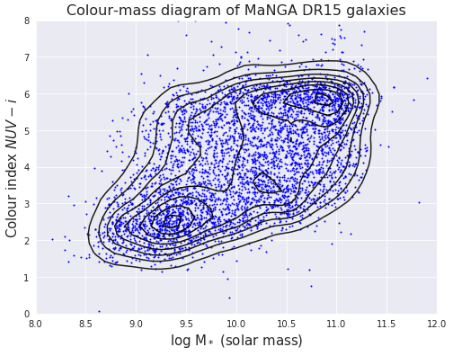
\includegraphics[width=\columnwidth]{images/CMDs/Colour-Mass-DR15-All.png}
    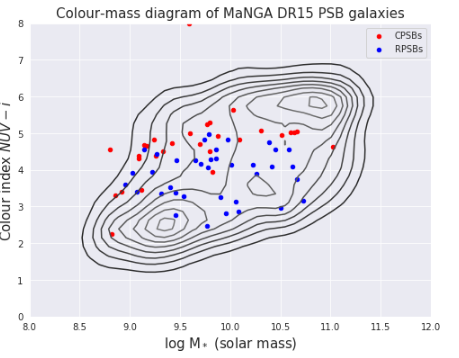
\includegraphics[width=\columnwidth]{images/CMDs/Colour-Mass-DR15-PSBs.png}
    \caption{We construct colour-mass diagrams for the full MaNGA DR15 survey population over a contour plot same this full sample (left panel). The our sample of PSBs is plotted over the same contour with the PSB galaxies plotted as points for CPSB sample (red dots) and RPSB sample (blue dots).}
    \label{fig:Colour-Mass-PSBs}
\end{figure*}


\subsection{Control galaxies}
\label{sec:controls}
A control sample set of regular galaxies not exhibiting PSB features was selected by Chen et al. (2019) sample. The purpose of the control sample is to provide a reference set of properties for comparison with the PSB data with a view to identifying typical progenitors which have not (yet) experienced a major merger. For each PSB, (CPSBs and RPSBs), a set of 10 non-PSB galaxies were selected but having similar stellar mass and global D$_n$4000 spectral indices. We used this control galaxy sample in this work.

[TODO: revise the caption in Figure \ref{fig:Colour-Mass-PSBs-controls} and ]

\begin{figure*}
    \centering
    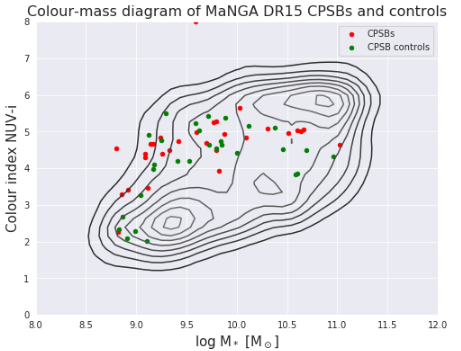
\includegraphics[width=\columnwidth]{images/CMDs/Colour-mass-CPSB+controls.png}
    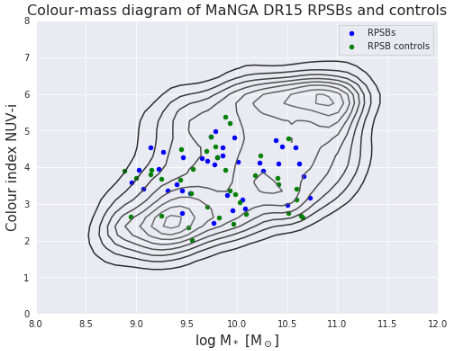
\includegraphics[width=\columnwidth]{images/CMDs/Colour-mass-RPSB+controls.png}
    \caption{Similar to Figure \ref{fig:Colour-Mass-PSBs}. The distribution of PSBs and their control galaxies has been laid over the the colour-mass contour plot of the full DR15 sample. In the left panel we have the distribution for the CPSB sample (red dots) with their control galaxies (green dots), in the right panel the RPSB sample (blue dots) with their corresponding controls (green dots).}
    \label{fig:Colour-Mass-PSBs-controls}
\end{figure*}

[TODO: add some text to highlight that the CPSBs and their controls are redward of the RPSBs.]

\subsection{PSB spectra}
The spectrum of a PSB galaxy exhibiting central PSB features is shown in Figure \ref{fig:CPSB-8623-9102-spec}.
\begin{figure*}
    \centering
    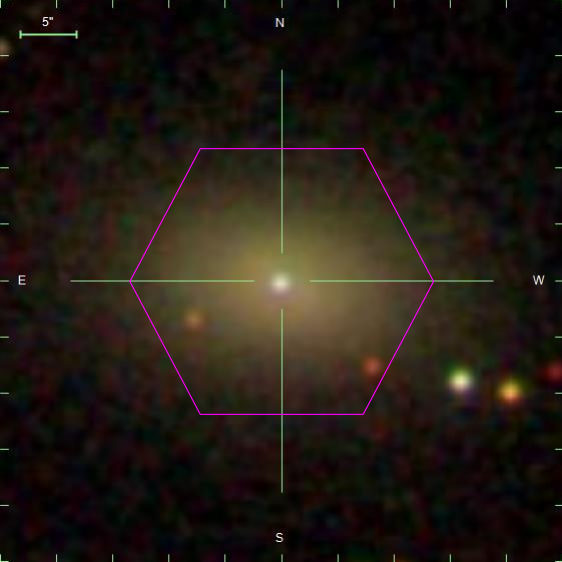
\includegraphics[width=0.22\textwidth]{images/Cutouts/CPSB-8623-9102-IM.png}
    \hfill
    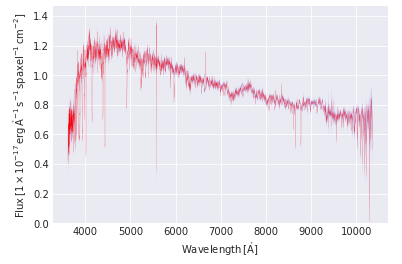
\includegraphics[width=0.38\textwidth]{images/Spectra/CPSB-8623-9102.png}
    \hfill
    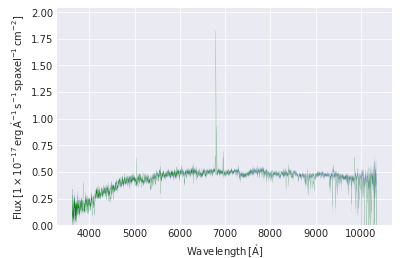
\includegraphics[width=0.38\textwidth]{images/Spectra/CPSB-CTRL-8990-3703-spec.png}
    \caption{Left: SDSS 3-colour image of central-type PSB 8623-9102. 
    Centre: The observed frame spectrum of the central spaxel of CPSB  8623-9102. Note the strong 4000 \AA\ break feature and strong hydrogen absorption lines in the wavelength region 3500 to 4500 \AA.
    Right: Observed frame spectrum of the control galaxy 8990-3703 with similar stellar mass to 8623-9102. This control galaxy shows relatively weak absorption lines and exhibits a strong H$\alpha$ emission line indicating the presence of cold gas and ongoing star formation.}
    \label{fig:CPSB-8623-9102-spec}
\end{figure*}


The spectrum of a ring-type RPSB galaxy exhibiting non-central PSB features is shown in Figure \ref{fig:RPSB-8323-6103-spec}.
\begin{figure*}
    \centering
    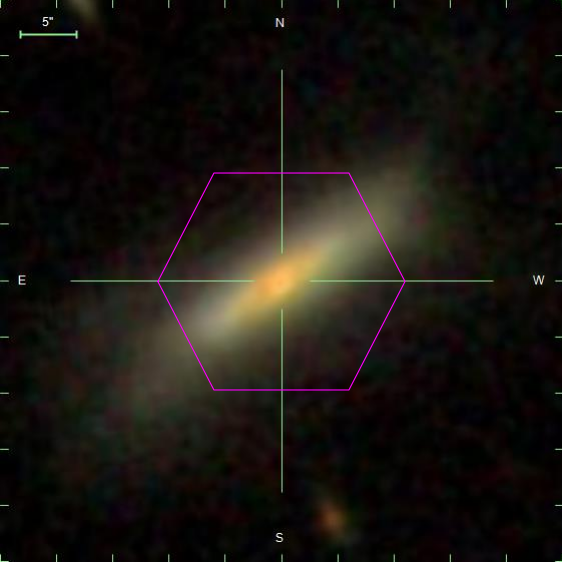
\includegraphics[width=0.24\textwidth]{images/Cutouts/RPSB-8323-6103-IM.png}
    \hfill
    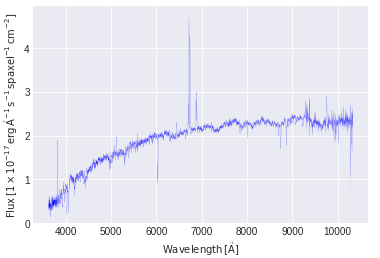
\includegraphics[width=0.35\textwidth]{images/Spectra/RPSB-8323-6103-27-27.png}
    \hfill
    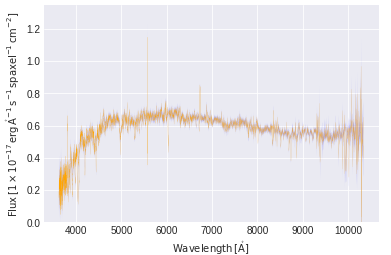
\includegraphics[width=0.35\textwidth]{images/Spectra/RPSB-8323-6103-34-32.png}
    \caption{Left: SDSS 3-colour image of the ring-type PSB 8323-6103. 
    Centre: The observed frame spectrum of the central region of ring-type PSB 8323-6103 at spaxel coordinates [27, 27] reveals strong H$\alpha$ emission consistent with an ample gas supply for continuing star formation.
    Right: The spectrum of ring-type PSB 8323-6103 at spaxel coordinates [34, 32], above and right of centre. The spectrum in this region exhibits the post-starburst features of weak emission lines, indicating a lack of gas, and strong Balmer absorption lines typical of the stellar atmospheres of A-type stars.}
    \label{fig:RPSB-8323-6103-spec}
\end{figure*}

An example of the MaNGA stellar velocity and gas velocity maps for a CPSB is illustrated in Figure \ref{fig:CPSB-8313-6101-VMAPS}.

\begin{figure}
    \centering
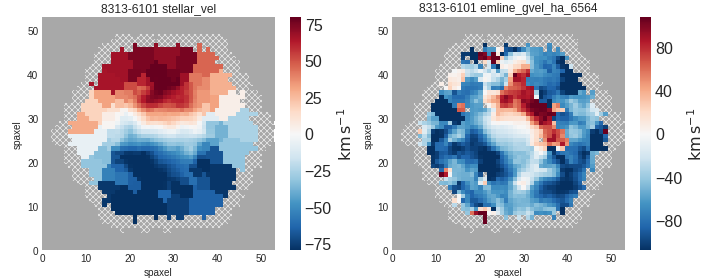
\includegraphics[width=\columnwidth]{images/VelocityMaps/CPSB-8313-6101-VMAPS.png}
    \caption{MaNGA velocity maps for CPSB 8313-6101: stellar velocity (left) and H$\alpha$ gas velocity (right).}
    \label{fig:CPSB-8313-6101-VMAPS}
\end{figure}

\subsection{Quality screening}
Global kinematic velocity position angles (PA) for the sample were determined using the \texttt{fit\_kinemetry\_pa} routine as described in appendix C of \cite{2006MNRAS.366..787K}. The routine returns the angle of the line bisecting the greatest change in velocity between the receding and approaching sides. \cite{2019MNRAS.483..172D} performed a \texttt{kinemetry} analysis of over 8,000 galaxies from the internal MPL-8 release of the MaNGA survey. In order to obtain a clean sample of well defined global PAs they visually classified the stellar and H$\alpha$ gas velocity fields of all galaxies in their sample into 3 categories (Chris Duckworth, 2019, personal communication), and set flags in their dataset as follows:

\begin{itemize}
    \item [1] Dominant coherent rotation and well defined PA. 
    \item [2] Dominant coherent rotation but with complex motions or highly inclined velocity fields 
    \item [3] Do not use
\end{itemize}

During this analysis galaxies with kinematically decoupled cores (KDCs) and warped velocity fields were also identified.

The resulting MPL-8 screened dataset from dataset of galaxies with reliable global PAs (flagged as [1] or [2]) from \cite{2019MNRAS.483..172D} was matched with the PSB galaxies in the sample of Chen et al. (2019, in prep.) to obtain a subset of PSBs with good \texttt{kinemetry} analysis flags. Furthermore a subset of those PSBs with $\Delta$PAs > 30\textdegree\ was extracted. The results are shown in Tables \ref{tab:my-CPSBs} and \ref{tab:my-RPSBs}. 

[Include a few examples of the PDF output from kinemetry: Chris' plots.]

In classical Kinemetry analysis it is considered significant if the $\Delta$PA position angle is greater than 30 degrees. We show some examples of misaligned stellar and gas velocity fields here: 
[TODO: tidy up this section.]

\begin{figure}
    \centering
    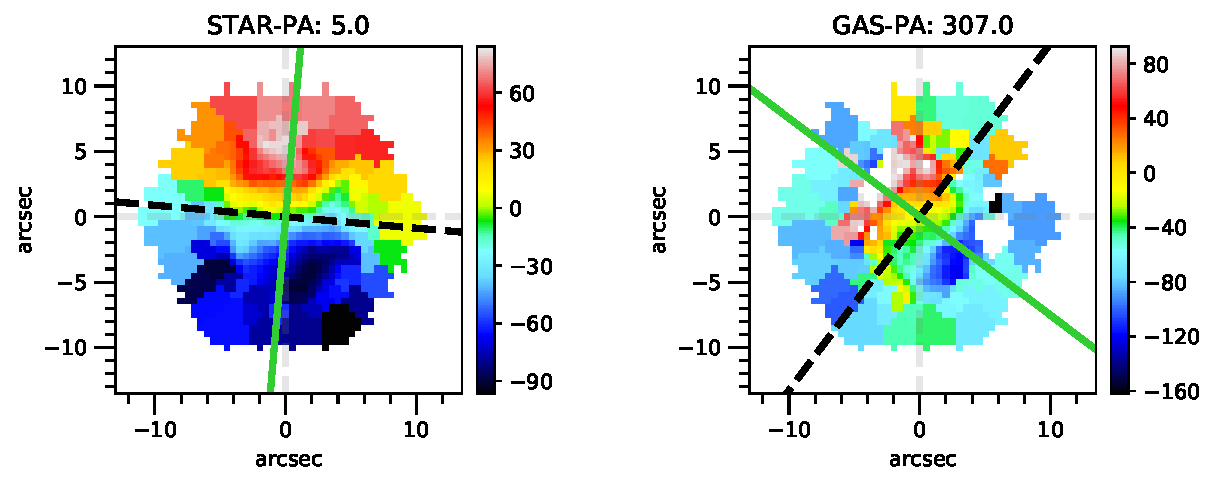
\includegraphics[width=\columnwidth]{images/PAplots/PAplotsCPSB/8313-6101-PA.pdf}
    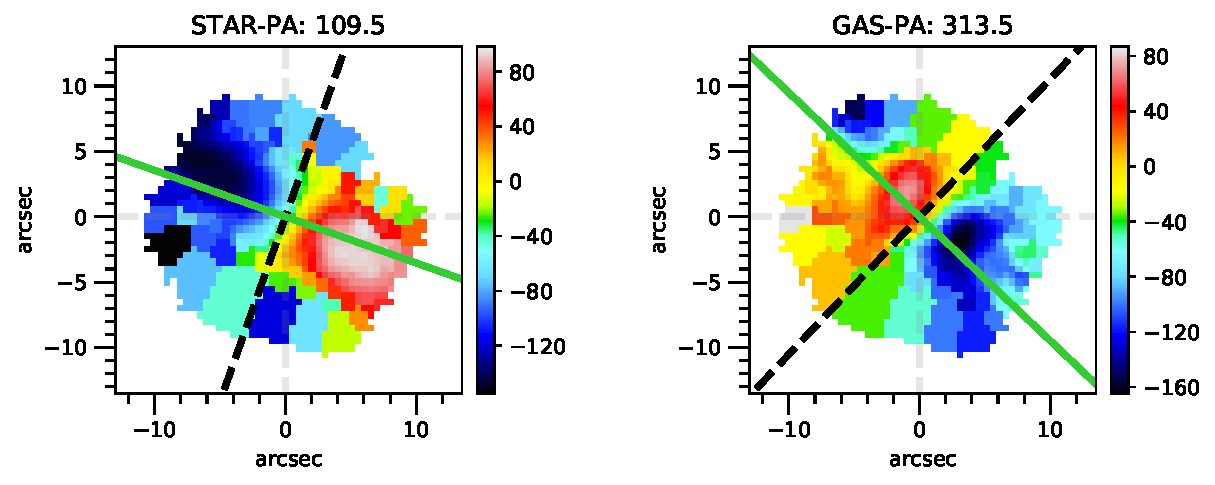
\includegraphics[width=\columnwidth]{images/PAplots/PAplotsRPSB/8323-6103-PA.pdf}
    \caption{Kinemetry-derived position angles (PA) for stellar velocity (left) and gas velocity (right) of two PSB galaxies exhibiting a significant $\Delta$PA. Top: CPSB 8313-6101, and bottom: RPSB 8323-6103. The velocity position angle is displayed as the green solid line while the black dashed line denotes the bisector of the velocity field between the receding (red) and blue (approaching) sides. The velocity colour scale is \kms. Credit for data analysis and plots: Chris Duckworth}
    \label{fig:CPSB-8313-6101-PA}
\end{figure}

\begin{table}
\caption{CPSBs with PA offset \textgreater 30 deg.}
\label{tab:offsetCPSBs}
\begin{tabular}{lccc}
\hline
PlateIFU  & Stellar PA & H$\alpha$ PA & $\Delta$PA \\
  & (deg.) & (deg.) & (deg.) \\
\hline
8313-6101 & 5 & 307 & 58 \\
8655-1902 & 335 & 127 & 152 \\
8725-1902 & 22 & 175 & 153 \\
8938-6102 & 214 & 47.5 & 166.5 \\
9494-3701 & 140.5 & 243 & 102.5 \\
\hline
\end{tabular}
\end{table}

\subsection{PA plots: misaligned RPSBs}

\begin{table}
\caption{RPSBs with PA offset \textgreater 30 deg.}
\label{tab:offsetRPSBs}
\begin{tabular}{lccc}
\hline
PlateIFU   & Stellar PA & H$\alpha$ PA & $\Delta$PA \\
  & (deg.) & (deg.) & (deg.) \\
\hline
8080-3704 & 24 & 154 & 130 \\
8262-3701 & 153.5 & 118.5 & 35 \\
8323-6103 & 109.5 & 313.5 & 156 \\
8439-6104 & 5.5 & 107 & 101.5 \\
8453-3704 & 44 & 91 & 47 \\
8486-1901 & 295.5 & 85 & 149.5 \\
8554-3701 & 250 & 68 & 178 \\
8932-12704 & 166.5 & 134.5 & 32 \\
9872-3701 & 208.5 & 81 & 127.5 \\
\hline
\end{tabular}
\end{table}



\section{Mergers and morphology}
\label{sec:mergers}

\subsection{Mergers and morphology}

Here we present a review of the literature on the detection of mergers and post-mergers, using morphology alone.

Galaxy morphology describes the transition of smaller, generally late-type normally disc galaxies from the so-called 'blue cloud' region of a galaxy colour-magnitude diagram (CMD) to large early-type elliptical galaxies distributed along the 'red sequence' region. Classical models describe a fast-track evolutionary phase transitioning from the blue cloud to the red sequence through a sparsely populated 'green valley' region of the galaxy CMD. An example of a galaxy CMD is shown in Figure \ref{fig:CMD-G_i-i}.

[JP guidance from VW: remove this when done]. Just so I don't forget: in your final report you will also need to include a section on how mergers and post-mergers are detected using morphology alone, perhaps 0.5-1 pages? A good place to start would be my former student Milena's papers: \citet{2016MNRAS.456.3032P} 
\citet{2018MNRAS.477.1708P} 
\citet{2019NatAs...3..440P} 
and this recent one from a MaNGA team member: \citet{2019ApJ...872...76N} 
As before, go up and down the ADS citations and references to ensure you have a complete literature review. 
I will leave this for you to do in your own time, once you have finished I'm happy to look over it. 

\section{Kinematics}
\label{sec:kinematics}

\citet{2015A&A...582A..21B} employed the Calor Alto CALIFA survey to study a sample of 103 interacting galaxies at various merger stages: close companions, systems with evidence of morphological interaction and coalesced merger remnants. Classification of the systems is performed by measuring the difference in kinematic position angles of the stellar and ionised gas velocity fields. A sample of 80 non-interacting galaxies was used as a control sample. The findings reveals that 42\% of interacting galaxies have a misalignment of over 16\textdegree\ while this is evident in only 10\% of the control sample.

[TODO: ]Make sure to reference \citet{2019MNRAS.483..172D}]


\subsection{kinemetry}
Kinemetry analysis employs the \texttt{kinemetry} software package developed by \citet{2006MNRAS.366..787K} to distinguish disc dominated systems from those exhibiting major mergers. The \texttt{Kinemetry} method involves mapping the gas velocity field and the gas velocity dispersion. Classification of a galaxy as a disc system or merger depends on the relationship between the gas velocity $v$ and the gas velocity dispersion $\sigma$.

\citet{2016A&A...591A..85B} examine the gas kinematics of nearby (ultra)luminous infrared galaxies ((U)LIRGs) at $z<0.1$. The objective is to analyse the kinematic properties of local (U)LIRGs to characterise their structures and thereby classify those (U)LIRGs as having disc structures (disc class), or displaying evidence of major merger activity (merger class). Their method employs optical integral field spectroscopy (IFS) data obtained at the VLT. H$\alpha$ emission is used as a gas velocity tracer. \citet{2016A&A...591A..85B} conclude that their results confirm that well-defined discs can be effectively distinguished from well-defined mergers but there is intermediate, indeterminate class. They note that the \texttt{kinemetry} method is sensitive to angular resolution of the integral field unit (IFU). \citet{2008ApJ...682..231S} had earlier performed an  analysis of warm gas kinematics as traced by H$\alpha$ emission, but concentrated on sample at $z\sim2$ using the NIR IFS instrument SIMFONI on the VLT. 


%% \section{Methods}
\label{methods}

\subsection{Kinemetry}





\subsection{Radon transform}

The global position angles obtained from the \texttt{kinemetry} method are well defined for coherently rotating stellar or gas velocity fields. In cases where galaxies exhibit radial variation in the velocity fields due to warps, where the velocity field in the outer regions is tilted compared with the core, in kinematically decoupled cores (KDCs), or in local regions of irregular velocity distribution the global PA does not provide a clear-cut description of the velocity field. A finer level of detail of the radial variation of the velocity field be accomplished using the Radon transform method. 
 Empty outline..

\section{Radon transform analysis}
\label{sec:methods-II-Radon}

\subsection{Motivation}
\label{sec:motivation}

Many galaxies display kinematic features in their morphology such as warps, kinematically decoupled cores (KDCs), bars, oval distortions, tidal tails etc. The global kinematic $\Delta$PA${k}$ is single number value, representing a broad average for the the entire galaxy. Finer details of any radial variation across a velocity field can be obtained using the \textbf{Radon transform} method.

In addition, PSBs have depleted their gas and star formation has shut down. The differential kinematic position angles $\Delta$PA${k}$ cannot be easily measured in gas-poor galaxies like our PSBs. However the Radon transform method can be applied to either or both the gas and stellar velocity fields. For our purposes we apply the Radon transform to the stellar velocity maps (only) of gas-poor PSBs. 


\subsection{Description of the Radon transform}

The Radon transform (RT) is a mathematical transformation of an image devised to reveal internal properties of an object such as structure. The transform method was originally devised by Johann Radon in 1917 \citep{radon1917determination}. Since then the technique has been applied to many fields, including various branches of astronomy including microwave, radio and x-ray applications. \citet{deans2007radon} describes many of these applications. The book also includes an English translation of Radon's original German text. In another work the PhD thesis of  Peter Toft \citet{7910dc8d5b654c90ac4bc94c67d06f01} promotes the application of Radon transforms in the field of digital signal processing and presents algorithms for its implementation. For our present purposes \cite{2018MNRAS.480.2217S} describe the application of the Radon transform method to galaxy kinematic studies. They developed IDL code routines to analyse the kinematic properties of stellar and gas velocity fields obtained from the MaNGA integral field survey. The objective is to quantify radial variations in the kinematic position angles (PA$_{k}$).

\begin{figure}
    \centering
    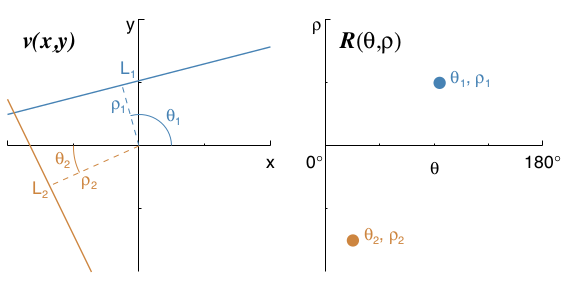
\includegraphics[width=\columnwidth]{images/RadonPlots/Radon-transform-Stark.png}
    \caption[The Radon transform and its coordinate system]{The Radon transform: illustration of the Radon transform and its coordinate system taken from Figure 1 in \citet{2018MNRAS.480.2217S}. Line integrals across a 2-D image in x,y coordinate space are calculated along all possible lines, parameterised by the coordinates [$\theta$, $\rho$]. The left panel shows examples of two solid lines, L$_1$ and L$_2$, which are mapped through the Radon transform function to points $\theta_1$, $\rho_1$ and $\theta_2$, $\rho_2$ in [$\theta$, $\rho$] parameter space in the right-hand panel. Credit: Stark et al. 2018.}
    \label{fig:RadonTransform}
\end{figure}

Mathematically the Radon Transform, $R$, is defined as
\begin{equation}
    \label{eqn:radon}
    R(\rho,\theta)=\int_{L}{v(x,y)\, \diff l},
\end{equation}

where $v(x,y)$ is a 2D velocity field defined in Cartesian coordinates and $\int_{L}$ is the line integral at transform sky-plane polar coordinates ($\rho,\theta$). This transform is illustrated graphically in Figure \ref{fig:RadonTransform} where lines through an image in 2D velocity space are mapped to a series of points in Radon transform [$\theta,\rho$] space by means of line integrals at various angles about the velocity space axes, and at various radial distances offset from the velocity space origin. 


\citet{2018MNRAS.480.2217S} apply a modification to the Radon transform, to obtain the \textit{Absolute} Radon Transform, as defined in Equation (\ref{eqn:radon}), by taking the integral of the absolute values of the velocity field difference of each point $v(x_i,y_i)$ and the mean of all values along the line segment.

\begin{equation}
    \label{eqn:radon_absolute}
    R_A=\int{| v(x,y) - \langle v(x,y) \rangle | \, \diff l}.
\end{equation}

There is another variant to the Absolute Radon Transform described by \citet{2018MNRAS.480.2217S} named the \textit{bounded}, or aperture restricted, Radon transform, R\textsubscript{AB}. Briefly, R\textsubscript{AB} involves placing integration limits $(\pm{r_{ap}})$, known as the aperture, on the integral of Equation \ref{eqn:radon_absolute} in order to limit the number of spaxels across a velocity map that will be used in the integration. \citet{2018MNRAS.480.2217S} developed a set of IDL (Interactive Data Language) algorithms to calculate the Radon transform on an input array representing a velocity field. The Radon transform IDL code is available on GitHub\footnote{\href{https://github.com/dvstark/radon-transform}{https://github.com/dvstark/radon-transform}}. 
The graphical output of the Radon transform code as applied to a synthetic velocity field is shown in Figure \ref{fig:Radon}.

\begin{figure}
    \centering
   	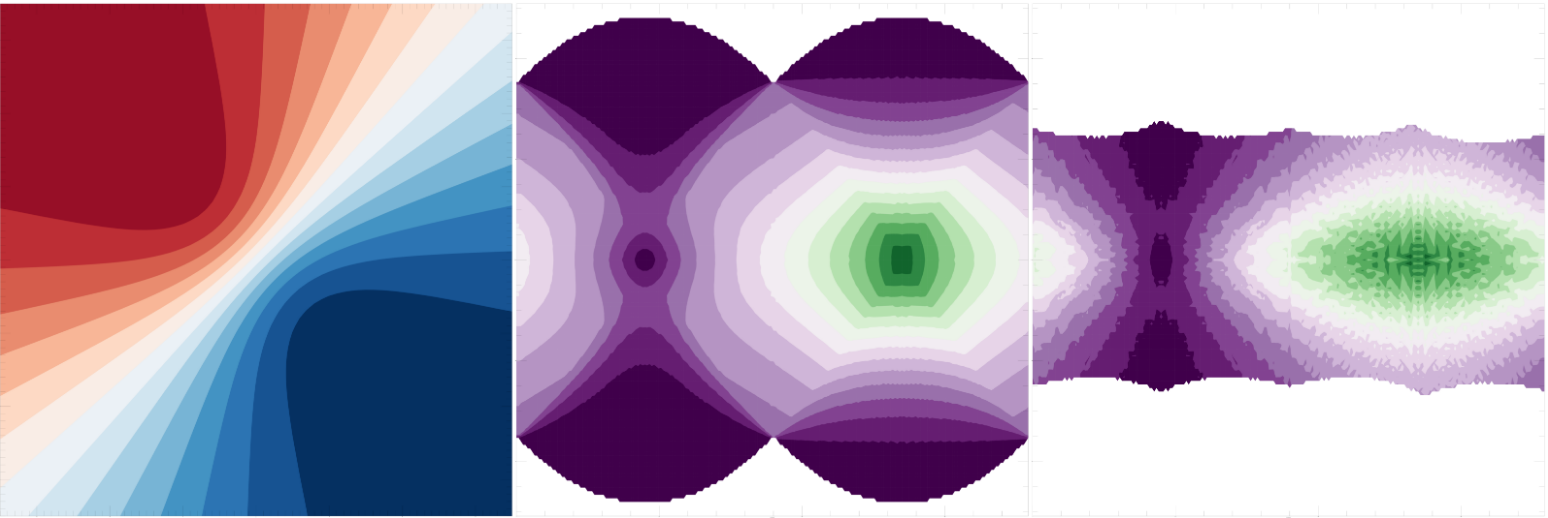
\includegraphics[width=\columnwidth]{images/RadonPlots/example.png}
    \caption[Model velocity field Radon transform plots]{Example of Radon transform code output for a model velocity field obtained by running the Radon example code publicly available on David Stark's GitHub website. The left panel shows a synthetic uniform velocity field model, the middle panel shows the the absolute Radon transform of the velocity field and the right panel shows the aperture-restricted absolute transform. We are concerned with the latter, the absolute aperture-restricted Radon transform of stellar and gas velocity fields in this work. Credit: David Stark.}
    \label{fig:Radon}
\end{figure}

Following \citet{2018MNRAS.480.2217S} we demonstrate the application of the Radon transform to stellar and gas velocity field data obtained from the SDSS-IV MaNGA integral field survey for a selection of CPSB and RPSB galaxies. The Radon transform output for the stellar (left) and gas (right) velocity fields of the central PSB 8131-6101 is shown in Figure \ref{fig:RT_8131-6101}. High velocity regions are indicated in green and low velocity areas in purple. The stellar velocity Radon transform plot (left) reveals a well defined minimum track across the radial (vertical) coordinate, again shown in purple. Notably the right hand panel showing the gas velocity transform reveals few features, possibly due to a sparsity of gas in CPSB 8131-6101.

\begin{figure}
    \centering
   	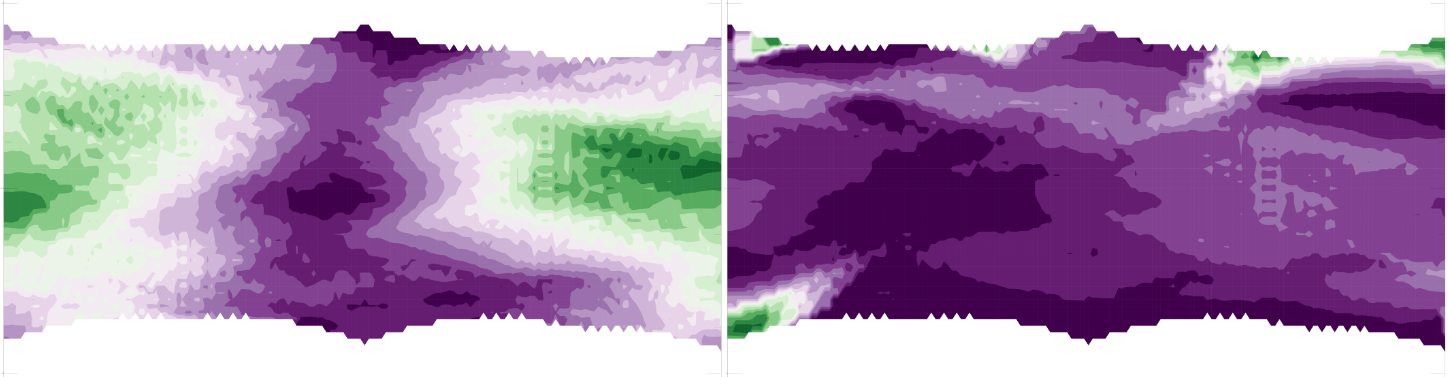
\includegraphics[width=\columnwidth]{images/RadonPlots/RT-snips/CPSB-8313-6101-RT-snip.png}
    \caption[Example of basic Radon transform plots for gas and velocity fields of CPSB 8131-6101]{Radon transform plots of the stellar velocity (left panel) and gas velocity (right) fields of CPSB of MaNGA PLATEIFU 8131-6101.}
    \label{fig:RT_8131-6101}
\end{figure}

% 

\begin{figure}
    \centering
    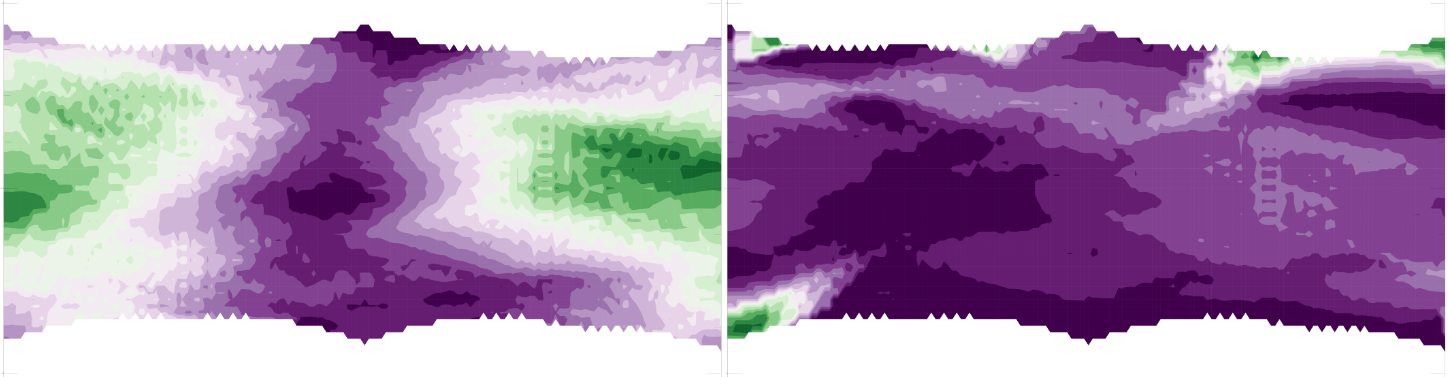
\includegraphics[width=\columnwidth]{images/RadonPlots/RT-snips/CPSB-8313-6101-RT-snip.png}
    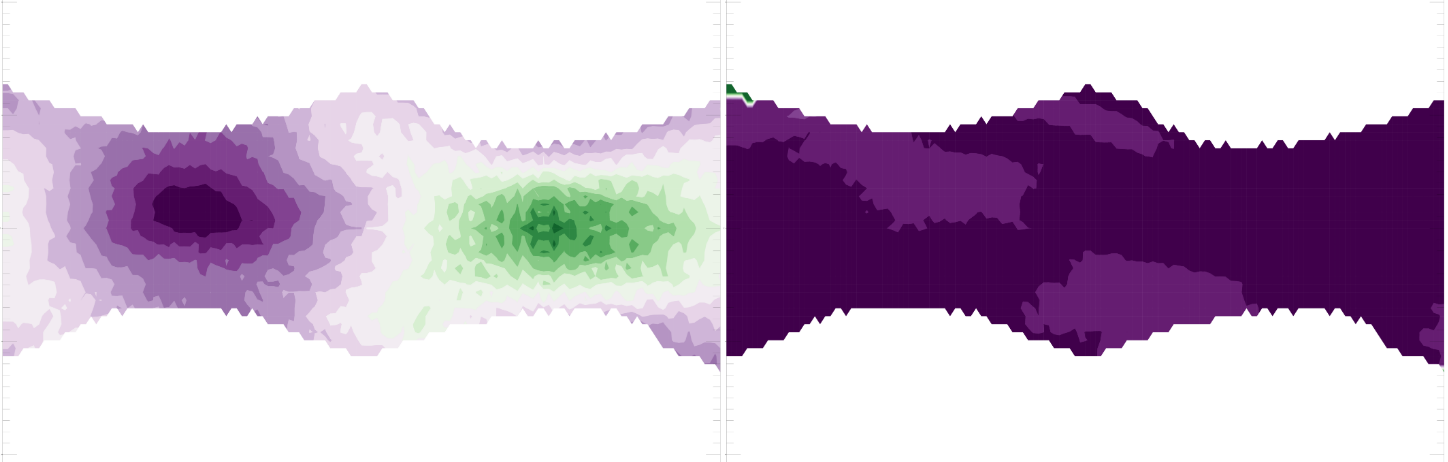
\includegraphics[width=\columnwidth]{images/RadonPlots/RT-snips/CPSB-9494-3701-RT-snip.png}
    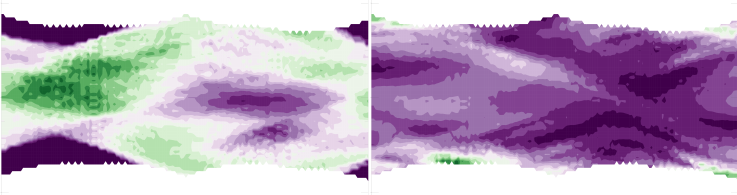
\includegraphics[width=\columnwidth]{images/RadonPlots/RT-snips/CPSB-8398-6102-RT-snip.png}
    \caption{CPSBs: Radon transforms of stellar velocity and gas velocity maps. From the top CPSB-8313-6101, CPSB-9404-3710 and CPSB -8398-6103}
    \label{fig:CPSB-RTs}
\end{figure}

\begin{figure}
    \centering
    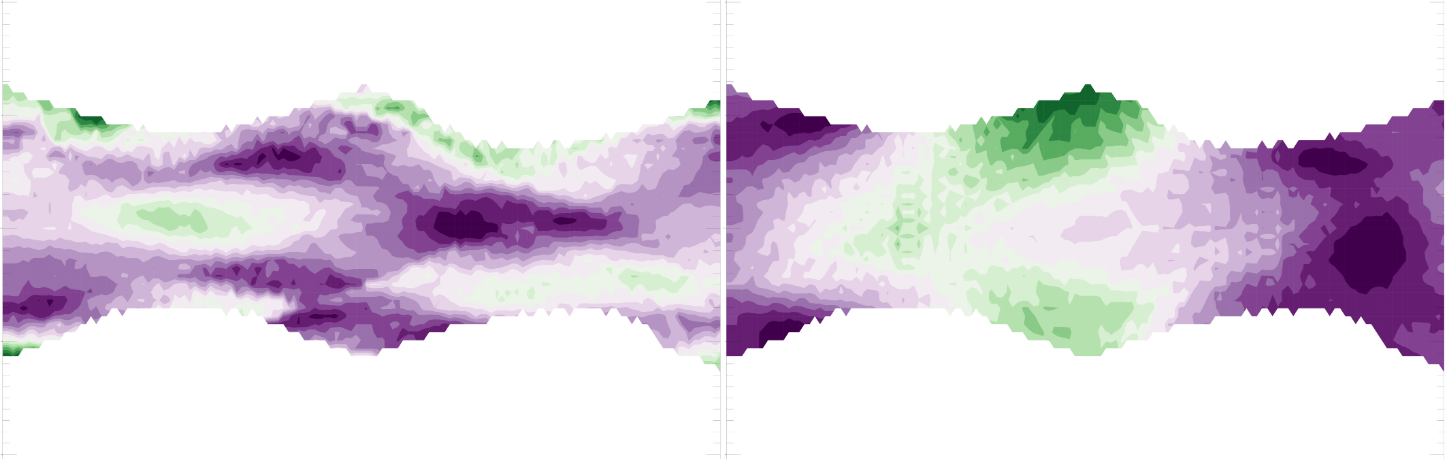
\includegraphics[width=\columnwidth]{images/RadonPlots/RT-snips/RPSB-9872-3701-RT-snip.png}
    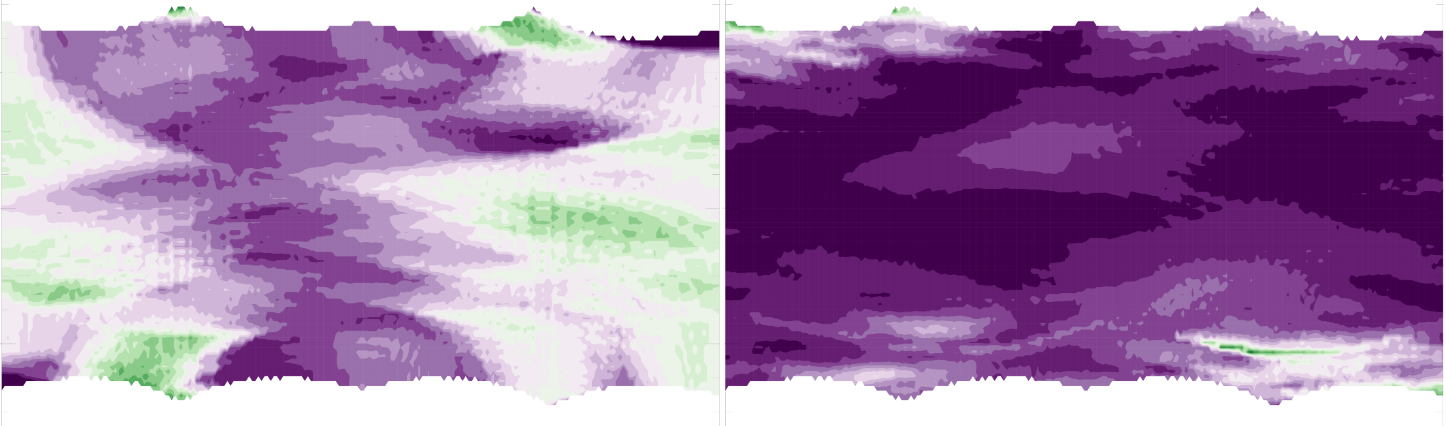
\includegraphics[width=\columnwidth]{images/RadonPlots/RT-snips/RPSB-8932-12704-RT-snip.png}
    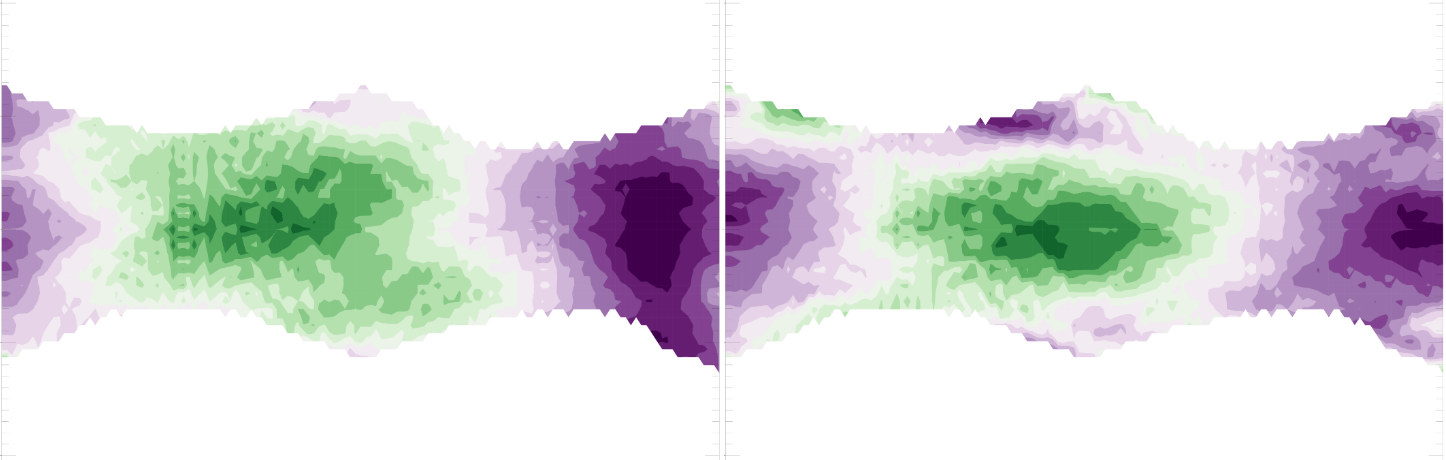
\includegraphics[width=\columnwidth]{images/RadonPlots/RT-snips/RPSB-8554-3701-RT-snip.png}
    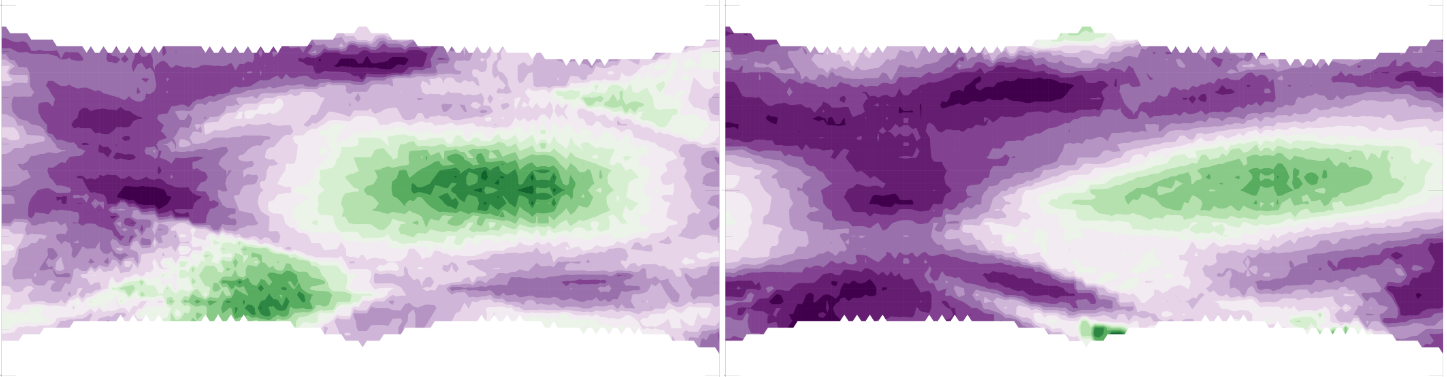
\includegraphics[width=\columnwidth]{images/RadonPlots/RT-snips/RPSB-8323-6103-RT-snip.png}
    \caption{Caption}
    \label{fig:RPSB-RTs}
\end{figure}   %% DO WE NEED THIS?

\subsection{Radon profile classification procedure}
\label{sec:Radon-classification}

\cite{2018MNRAS.480.2217S} identified 5 commonly recurring patterns in the stellar and gas velocity field Radon transform profiles of their MaNGA galaxy sample. These patterns were used to classify the computed Radon trace profiles. In this project work we adopt the same classification approach for the Radon profiles of our PSB galaxies and their control samples. Simplified models of 4 of the trace profile classes are shown in Figure \ref{fig:class-models}. In addition an asymmetric profile class was identified. Detailed examples of the trace profile class types are presented in Figure 7 of \cite{2018MNRAS.480.2217S}. The salient features of these 5 Radon profile classes are listed below:

\begin{itemize}
    \item Constant, \textbf{Type-C} : Radon profile with relatively constant trace minimum angle $\hat{\theta}$ at all radii $\rho$.
    \item Inner Bend, \textbf{Type-IB} : Galaxies whose Radon profiles exhibit symmetrical variations of $\hat{\theta}$ beginning at $|\rho|=0$, then transitioning to a constant value. 
    \item Outer Bend, \textbf{Type-OB} : Galaxies with constant Radon trace angle $\hat{\theta}$  at small $|\rho|$ which transition to a different value at a greater radius. 
    \item Inner Bend + Outer Bend, \textbf{Type-IB+OB} : Galaxies with Radon profiles showing a combination of the features of Type-IB and Type OB profiles.
    \item Asymmetric, \textbf{Type-A} : The value of the $\hat{\theta}$ varies significantly with $\rho$ across opposite sides of the transform R\textsubscript{AB}. 
 \end{itemize}

\begin{figure}
    \centering
    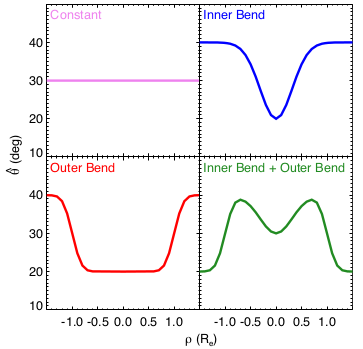
\includegraphics[width=0.8\columnwidth]{images/RadonPlots/Radon-class-models.png}
    \caption[Radon profile class feature identification: toy models]{Toy models of the Radon profile (trace angle minimum $\hat\theta$ versus radius $\rho$). The sub-plots display examples of 4 of the Radon profile classes used for classification of the RT trace plots. Upper left: Constant, Type-C; upper right: Inner Bend, Type-IB; lower left: Outer Bend, Type-OB; and lower right: Inner Bend + Outer Bend, Type-IB+OB. Source: Stark et al. (2018) figure 8.}
    \label{fig:class-models}
\end{figure}

Mathematical functions describing these Radon profile classifications have been identified by \citet[][section 3.6]{2018MNRAS.480.2217S}. This has enabled code routines to be developed which can provide automatic classification of the Radon trace profiles. Results of the automatic classification routines were made available quite late on during the progress of the project work, and therefore were not used extensively in this analysis. Instead, we have adopted a simple visual classification method to categorise each of our sample galaxy into one of the 5 Radon profile trace types listed above. Visual classifications were determined by following a 3-step process:

\begin{enumerate}
    \item Firstly we obtain the MAPS data cube FITS files for the selected PSB galaxies listed in Tables \ref{tab:my-CPSBs} and \ref{tab:my-RPSBs}, and a similar number of 'normal' galaxies drawn from their respective control samples, as described in Section \ref{sec:controls}, downloaded from the MaNGA website.
    \item Next, we process each of data cubes through the Radon transform wrapper code to obtain graphical output files showing the galaxy SDSS $gri$ image cutout, the MaNGA stellar velocity map, the absolute bounded Radon transform R\textsubscript{AB} plot and the Radon profile plot of $\hat{\theta}$ versus $\rho$. An example of this output for the CPSB galaxy 8979-1902 is shown in Figure \ref{fig:CPSB-8979-1902-SNIP}. 
    \item  We then examine the output plot for each galaxy to  visually assess the relative qualitative strength of each of the 5 classification features by assigning a numeric weighting as given in Table \ref{tab:features}. This method adds a semi-quantitative approach to the visual assessment process.
\end{enumerate}

\begin{figure*}
    \centering
    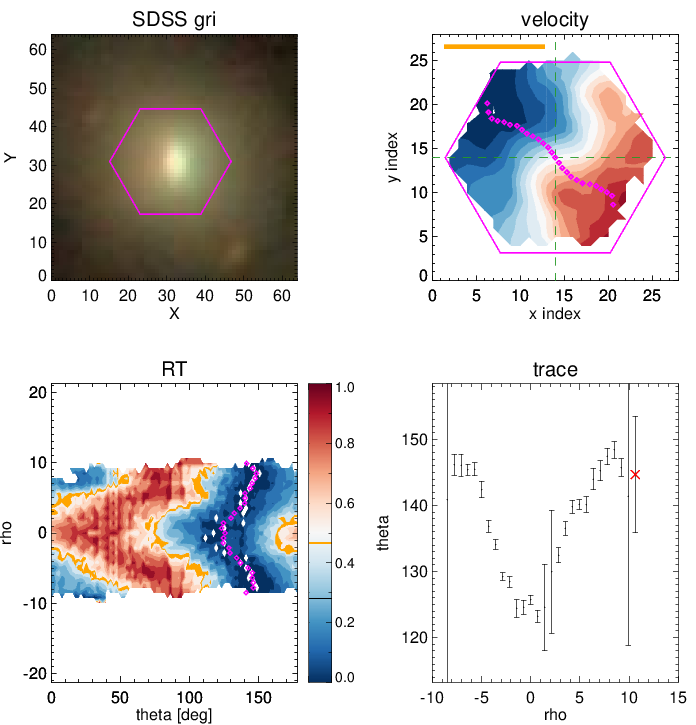
\includegraphics[width=0.8\textwidth]{images/RadonPlots/RT-SNIPS-NEW/CPSB-8979-1902-SNIP.png}
    \caption[Radon transform code output graphics for the CPSB 8979-1902]{Radon transform code output graphics for the CPSB 8979-1902. Top left: SDSS gri image cutout, Top right: stellar velocity map with kinematic position angle (PA$_{k}$) shown as the magenta line, lower left: Radon transform (RT) of the stellar velocity field with the transform minimum angle $\hat\theta$ plotted across radius $\rho$ in magenta, lower right: the Radon profile trace of the RT minimum.}
    \label{fig:CPSB-8979-1902-SNIP}
\end{figure*}

\begin{table}
    \caption[Relative weighting of Radon profile feature strengths used in visual classification]{Relative weighting of Radon profile feature strengths used for the visual classification of Radon profile feature types: Constant, Inner Bend, Outer Bend, Inner Bend + Outer Bend or Asymmetric. The weighting is assigned to help quantify the visual appearance of the trace profile plots.}
    \label{tab:features}
    \centering
    \begin{tabular}{cl}
    \hline
    Value & Visual appearance \\
    \hline
    2 & The feature is visually predominant \\
    1 & Some evidence of the feature is apparent \\
    0 & The feature is absent \\
    \hline
    \end{tabular}
\end{table}

The Radon output graphic plots for 127 galaxies (PSBs and some of control sets) were visually assessed in alphanumerical order of their PLATEIFU file name tag, which effectively creates a random sequence across the groups. Classifying the galaxies in each group sequentially may have led to preferential identification of similar features in that group, thereby introducing a classification bias.

The Radon transform output plots for each galaxy were inspected to make an assessment of the visual strength of each of the Radon profile type features evident. A numerical value 0, 1 or 2, representing the visual strength of apparent features from Table \ref{tab:features}, was assigned to each of the 5 predefined Type classes for the galaxy. Based on the relative strength values allocated, a predominant feature Type (C, IB, OB, IB+OB or A) was assigned to that particular galaxy. To determine the relative predominance of Type-IB+OB features we simply summed the strength values assigned to Types IB and OB together. 
In many cases there was ambiguity in the absolute Type assessment, where we had difficulty to select only one of the 5 predefined classes. In these cases a secondary assessment was made, generally this was the most prevalent Type plus a sub-dominant feature. The secondary assessment was intended to be used later to refine the analysis process. 

As a demonstration of the Radon profile visual classification method we select the example of the spiral galaxy 8979-12701. The Radon transform and Radon profile trace for this galaxy are shown in Figure \ref{fig:OB+IB}. Comparing the Radon trace profile with the model traces in Figure \ref{fig:class-models} and the examples given in  Figure 7 of \cite{2018MNRAS.480.2217S}, the visual classification process identified the strength of the features as: C = 1, IB = 2, OB = 2, IB+OB = 2+2 = 4, and A=0. This trace profile is comparable to the Type-OB+IB model and consequently the Radon profile of this galaxy is categorised as Type-OB+IB.

The classification process outlined above was carried out independently by 2 persons in an endeavour to provide some means of eliminating personal subjectivity. The intent is similar  to that adopted by the Galaxy Zoo project which used large-scale public collaboration to classify galaxy morphology \citep{2017MNRAS.464.4176W}. The galaxy-by-galaxy Radon profile Type classifications determined by the two assessors are listed in Tables \ref{tab:full-visual-classification} and \ref{tab:visual-classification-B} in Appendix \ref{sec:visual-classification-tables}.

\begin{figure}
    \centering
    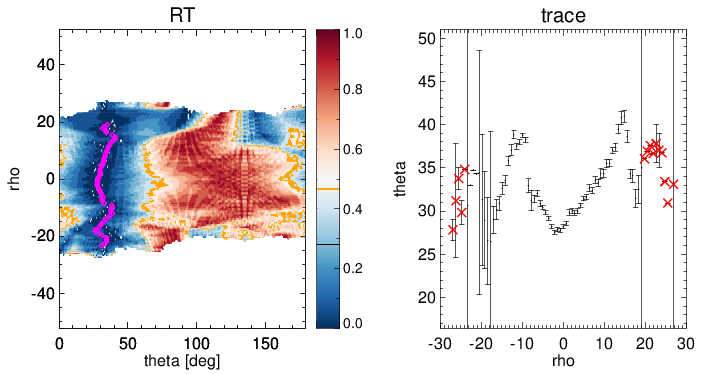
\includegraphics[width=\columnwidth]{images/RadonPlots/RT-SNIPS-NEW/8979-12701-VA-OB+IB.png}
    \caption[Example of the Radon profile visual classification of galaxy 8979-12701]{Example of the Radon profile visual classification method for galaxy 8979-12701. The Radon transform (RT) plot is shown in the left panel and the Radon profile trace on the right. The RT plot minimum (magenta line) shows an indication of a wide outer bend (OB) feature. The trace plot also shows a narrower inner bend (IB) feature centred at radius $\rho=0$. We therefore classify the Radon profile of this galaxy as Type-OB+IB.}
    \label{fig:OB+IB}
\end{figure}

During the classification assignment exercise  some difficulties were encountered mainly with Radon trace profiles that did not fit easily into on of the 5 classification Types. An example of this is seen in the case of 8555-3701 where a clearly defined Inner Bend appears superimposed on an asymmetric trace as shown in Figure \ref{fig:8555-3701-A+IB}. The form of this trace does not fall readily into either of the Type-A or Type-IB categories, however faced with a choice of Types, and a requirement to select only one of the 5 categories, the natural choice was to opt for the predominant feature, in this case Type-A, asymmetric. The reader may disagree and opt for Type-IB, or even Type-OB+IB. This demonstrates the challenges encountered in the visual classification of Radon profiles.

\begin{figure}
    \centering
    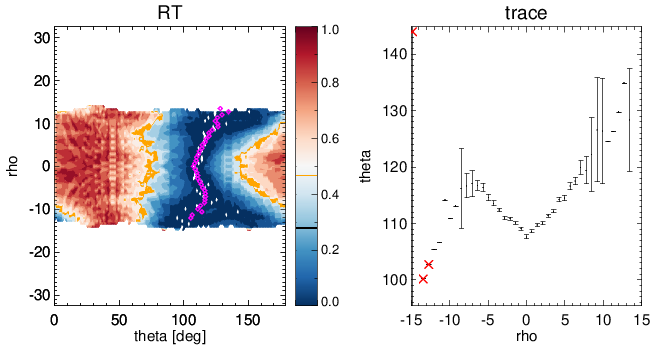
\includegraphics[width=\columnwidth]{images/RadonPlots/RT-SNIPS-NEW/8555-3701-A+IB.png}
    \caption[Radon transform and profile trace plots for the galaxy 8555-3701]{Radon transform and profile trace plots for the galaxy 8555-3701. An inner bend appears superimposed on a generally asymmetric trace.}
    \label{fig:8555-3701-A+IB}
\end{figure}

In many other cases bends, or detectable velocity field disturbances, are evident as notches at well off-centre radii on otherwise constant or largely asymmetric traces. To obtain a comprehensive census at this level of detail these sub-dominant and off-centre features should be taken into account in a secondary analysis as mentioned above. Other than presenting a listing of the mixed secondary classifications obtained by classifier A in Table \ref{tab:full-visual-classification}, we did not pursue a more detailed secondary analysis in this present work.






%% RT-plots-new.tex
%% Images from the new Radon output 

\begin{figure*}
    \centering
    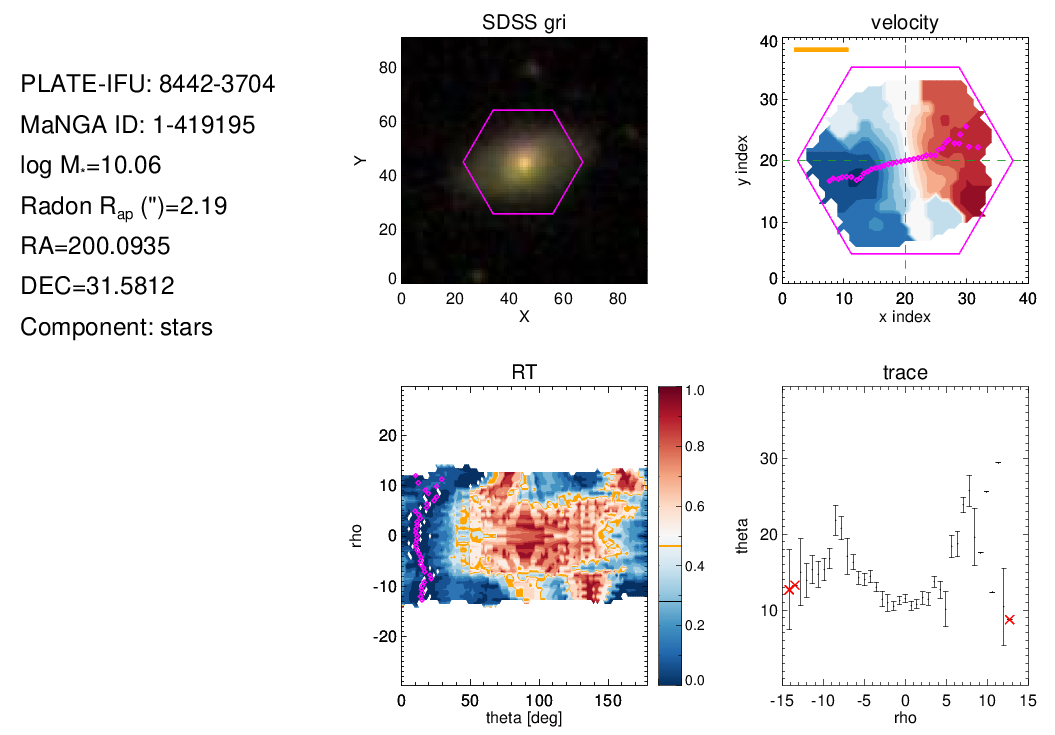
\includegraphics[width=\textwidth]{images/RadonPlots/RT-SNIPS-NEW/8442-3704-complete.png}
    \caption{The Absolute Radon transform code output graphics for stellar velocity field of the galaxy MaNGA PLATEIFU 8442-3704. The left side text block provides some relevant data about the galaxy extracted from the MaNGA DAP. The quadrature arrangement of panels to the right show: top left - the SDSS IFU gri image cutout; top right - the stellar velocity field with kinematic position angle PA\k superimposed by the magenta line. The orange coloured  bar in the upper left indicates the Radon aperture size in spaxels; bottom left - the absolute value of Radon transform re-scaled from 0 to 1. The locus of the minimum of the transform is plotted in magenta; and bottom right: the Radon trace plot.}
    \label{fig:8442-3704-complete}
\end{figure*}

This Radon transform code output for this particular galaxy, MaNGA ID 1-419195 plateifu 8442-3704, reveals some particularly significant stellar kinematic features, however at this point we have not classified the galaxy in terms of its Radon profile type. Radon profile classification will be discussed in some depth in Section \ref{sec:Radon-classification}.     %% REFERENCE THIS SOMEWHERE




\section{Results and analysis}
\label{sec:results}

In this section we present the results of the three main topic areas of our study of PSB galaxies and their kinematical properties:

\begin{itemize}
    \item Basic property distributions
    \item Kinematic position angle analysis
    \item Radon transform profile classification and analysis
\end{itemize}

\subsection{Basic property distributions}
\label{sec:property-distributions}
Initially we performed some cursory checks on the distributions of some basic properties of our galaxy samples. Here we present those results as histograms comparing characteristic properties of CPSBs, RPSBs and their control galaxies. We show distributions of CPSB properties alongside those of the RPSB sample in terms of the following 3 fundamental properties: 
\begin{itemize}
\item stellar mass
\item redshift
\item S\'ersic index
\end{itemize}
The frequency distribution histograms of these properties are plotted in Figures \ref{fig:stellar-mass-plot}, \ref{fig:redshift-plot} and \ref{fig:Sersic-plot} respectively. The data underlying these  distributions is drawn from the MaNGA \texttt{drpAll} catalogue. The specific property values for each PSB is listed in Appendix \ref{sec:lists-of-psbs}, Tables \ref{tab:my-CPSBs} and \ref{tab:my-RPSBs}.

\textbf{Stellar mass:} The distribution in stellar mass for the CPSBs is compared to that of the RPSBs in Figure \ref{fig:stellar-mass-plot}. Both PSB groups span a similar range in mass. This result was noted previously during the interpretation of the colour-mass diagram depicted in Figure \ref{fig:Colour-Mass-PSBs}.

\begin{figure}
    \centering
    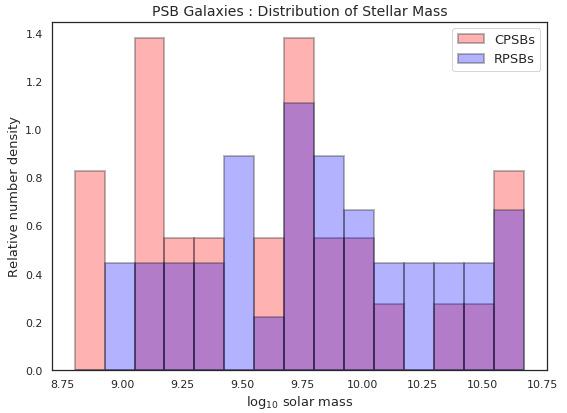
\includegraphics[width=\columnwidth]{images/JupyterPlots/Dist-Stellar-Mass-All.png}
    \caption[Distribution of stellar mass for CPSBs and RPSBs]{Distribution of stellar mass of our sample of CPSBs (red) and RPSBs (blue). On the logarithmic scale of $\log_{10}$\Msun\ a fairly uniform distribution of stellar mass is apparent for both populations, CPSBs and RPSBs.}
    \label{fig:stellar-mass-plot}
\end{figure}

\textbf{Redshift:} A comparison of the distribution in redshift for our CPSB and RPSB groups is shown in Figure \ref{fig:redshift-plot}. The redshift range of both groups lies in the range $0.01 < z < 0.08$. The shape of the redshift distribution of both groups is remarkably similar. We cannot distinguish the CPSB and RPSB populations based on redshift.

\begin{figure}
    \centering
    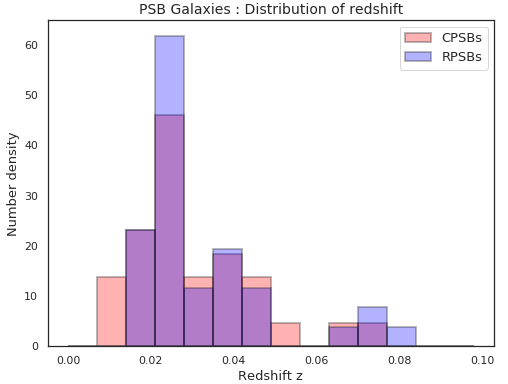
\includegraphics[width=\columnwidth]{images/JupyterPlots/Dist-z-All.png}
    \caption[PSB distribution in redshift]{Distribution in redshift z as obtained from the NSA.Z data value in the MaNGA \texttt{drpAll} file. The redshift distribution for the CPSB sample (shaded in red) is compared to that of the RPSB sample (blue).}
    \label{fig:redshift-plot}
\end{figure}

\textbf{S\'ersic index:} The surface brightness profile of a galaxy is generally a function of radius from the nucleus. The rate of change of brightness can be described by the S\'ersic function or S\'ersic index (SI). Low values of SI $\sim$1 relate to disc-type galaxies, whereas SI values of 3 or more are commonly measured in galaxies with compact bright nuclei indicative of more evolved systems. A wide range of S\'ersic index values is apparent in the distribution, as shown in Figure \ref{fig:Sersic-plot}, implying the presence of disparate morphologies in the sample. We note from the distribution that CPSBs tend to have higher S\'ersic index values than RPBs. This suggests that CPBs have more concentrated nuclei and a spheroidal morphology in contrast to the disc-like RPSBs with lower S\'ersic index values.

\begin{figure}
    \centering
    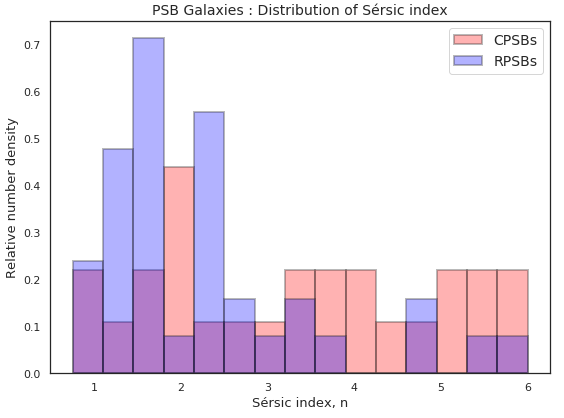
\includegraphics[width=\columnwidth]{images/JupyterPlots/Dist-Sersic-Index-All.png}
    \caption[Comparison of the distribution of S\'ersic index values of CPSBs and RPSBs]{Distribution of S\'ersic index (SI) values. The relative number density distribution of the S\'ersic index value for 26 CPSBs (red histogram) and 36 RPSBs (blue) are plotted. Five PSBs with unreliable SI values (SI = 6.000) in the NSA data  have been excluded.}
    \label{fig:Sersic-plot}
\end{figure}

In summary, the basic property distributions of CPSBs and RPSBs are very similar for stellar mass and redshift. The distribution of S\'ersic index does however reveal that RPSBs generally have lower SI values implying they are disc-like objects, while CPSBs with higher SI values indicate the morphology of spheroids.

%%%%====== Orphaned figures ======

\subsection{Kinematic position angle analysis}
\label{PA-misalignment}
The gas and velocity field position angle misalignment measurements for PSBs where the $\Delta$PA$_{k}$ \textgreater\ 30\textdegree\ are presented in Table \ref{tab:offsetCPSBs} for the CPSBs, and Table \ref{tab:offsetRPSBs} for the RPSBs. Here it can be seen that the number of PSBs having clearly defined $\Delta$PA$_{k}$ i.e. \textgreater\ 30\textdegree, is a small fraction of the PSB sample: 5 out of 30, or 17\% of CPSBs, and 9 out of 37, or 24\% of RPSBs. 

In contrast, looking at the control galaxies, the velocity field position angle variance of the CPSB and PSB control samples is shown in Figure \ref{fig:controlDeltaPAs}. Both sets of control galaxies have low values of velocity field $\Delta$PA$_{k}$, i.e. the stellar velocity and gas velocity fields are generally closely aligned.

\begin{table}
\centering
\caption{CPSBs with gas and stellar velocity kinematic PA offsets \textgreater 30\textdegree.}
\label{tab:offsetCPSBs}
\begin{tabular}{lccc}
\hline
PlateIFU  & Stellar PA & H$\alpha$ PA & $\Delta$PA \\
  & (deg.) & (deg.) & (deg.) \\
\hline
8313-6101 & 5 & 307 & 58 \\
8655-1902 & 335 & 127 & 152 \\
8725-1902 & 22 & 175 & 153 \\
8938-6102 & 214 & 47.5 & 166.5 \\
9494-3701 & 140.5 & 243 & 102.5 \\
\hline
\end{tabular}
\end{table}

\begin{table}
\centering
\caption[RPSBs with kinematic velocity PA offsets \textgreater 30\textdegree.]{RPSBs with gas and stellar velocity kinematic PA offsets \textgreater 30\textdegree.}
\label{tab:offsetRPSBs}
\begin{tabular}{lccc}
\hline
PlateIFU   & Stellar PA & H$\alpha$ PA & $\Delta$PA \\
  & (deg.) & (deg.) & (deg.) \\
\hline
8080-3704 & 24 & 154 & 130 \\
8262-3701 & 153.5 & 118.5 & 35 \\
8323-6103 & 109.5 & 313.5 & 156 \\
8439-6104 & 5.5 & 107 & 101.5 \\
8453-3704 & 44 & 91 & 47 \\
8486-1901 & 295.5 & 85 & 149.5 \\
8554-3701 & 250 & 68 & 178 \\
8932-12704 & 166.5 & 134.5 & 32 \\
9872-3701 & 208.5 & 81 & 127.5 \\
\hline
\end{tabular}
\end{table}

% \subsection{Distributions of kinematic position angles}
We now turn to analyse the distributions of the differential kinematic position angles $\Delta$PA$_{k}$ evident in our PSB samples and their control galaxies. Firstly, in Figure \ref{fig:deltaPAdistribution} we show the distribution of $\Delta$PA$_{k}$ in the CPSB sample versus the RPSB sample. This figure shows that CPSBs generally have higher $\Delta$PA$_{k}$ values than the RPSB population. This in an interesting finding in that CPSBs indicate a greater of misalignment between their gas and stellar velocity fields than RPSBs. If we consider past merger scenarios, this evidence may indicate that the masses of progenitor components are comparable in the CPSB distribution, but less so in the case of RPSB mergers.

\begin{figure}
    \centering
    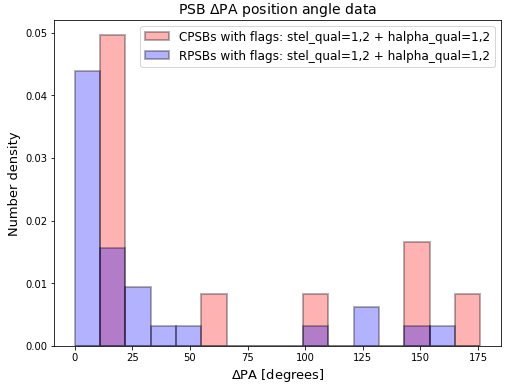
\includegraphics[width=\columnwidth]{images/JupyterPlots/Dist-Delta-PA-All-GoodFlags.png}
    \caption[Distribution of PSB stellar and gas velocity field position angles]{Distribution of PSB galaxy velocity field position separation angles ($\Delta$PA$_{k}$) for those PSBs with stellar velocity and gas velocity characteristics flagged as 'good' as denoted in the legend (see the text in Section \ref{sec:kinemetry-analysis-method-description} for details). CPSB $\Delta$PA$_{k}$ density weights are plotted in red, RPSB $\Delta$PA$_{k}$ weights in blue.}
    \label{fig:deltaPAdistribution}
\end{figure}

We now examine the distribution in kinematic position angle of the subject PSB groups: CPSBs, RPSBs and their respective control galaxy samples. The distribution in $\Delta$PA$_{k}$ of the CPSB sample against their control population is shown in Figure \ref{fig:CPSBvsControlDeltaPAs}. The CPSBs have significantly larger kinematic $\Delta$PA$_{k}$ than the control galaxy group.

\begin{figure}
    \centering
    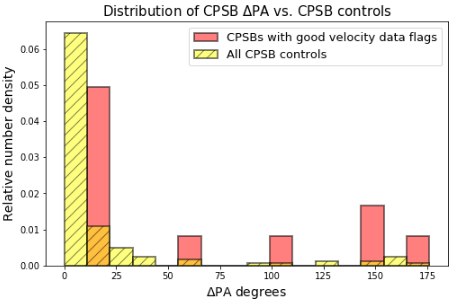
\includegraphics[width=\columnwidth]{images/JupyterPlots/DIST-DPA-CPSB+FLAGS+controls.png}
    \caption[Distribution of CPSB $\Delta$PA vs. their CPSB controls]{Distribution of CPSB stellar and gas velocity position angle difference $\Delta$PA vs. their CPSB controls. Note the CPSBs selected are a subset where their gas and stellar kinematic map data has been flagged as usable. CPSBs PA distributions are plotted in red with their CPSB controls in yellow with hatching. The PA offset in CPSB $\Delta$PA is discussed in the text.}
    \label{fig:CPSBvsControlDeltaPAs}
\end{figure}

The distribution in kinematic position angle of the RPSB sample against their control population is shown in Figure \ref{fig:RPSBvsControlDeltaPAs}. The RPSBs possess larger kinematic $\Delta$PA$_{k}$ than their control galaxy group, but to a lesser extent than the CPSBs to their controls. Significantly, we see an emerging trend: CPSBs exhibit larger kinematic $\Delta$PA$_{k}$ than the RPSB group.

To complete the picture, we look at the comparative distribution of the control galaxy $\Delta$PA$_{k}$ for both PSB groups: CPSBs and RPSBs. This is shown in Figure \ref{fig:controlDeltaPAs}. We note that the distributions of control galaxy $\Delta$PA$_{k}$ are very similar and bunched at less than 20\textdegree. 

\begin{figure}
    \centering
    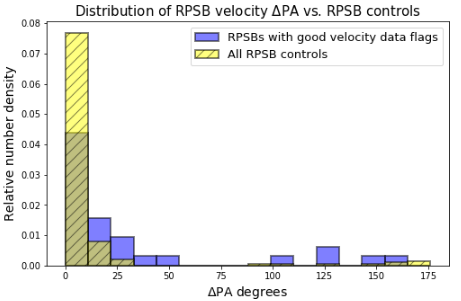
\includegraphics[width=\columnwidth]{images/JupyterPlots/DIST-Good-RPSB+Flags+Controls.png}
    \caption[Distribution of RPSB velocity $\Delta$PA vs. their RPSB controls]{Distribution of RPSB stellar and gas velocity $\Delta$PA vs. their RPSB controls. Note the RPSBs selected are a subset where their gas and stellar kinematic map data has been flagged as usable. RPSB PA distributions are plotted in blue with their RPSB controls in yellow with hatching}
    \label{fig:RPSBvsControlDeltaPAs}
\end{figure}


\begin{figure}
    \centering
    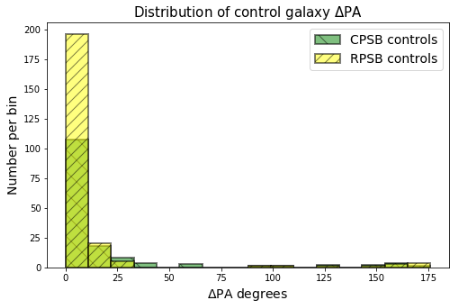
\includegraphics[width=\columnwidth]{images/JupyterPlots/DIST-Control-DPA-both.png}
    \caption[Distribution of control galaxy $\Delta$PA$_{k}$]{Distribution of both CPSB and RPSB control galaxy stellar and gas velocity field position angle difference $\Delta$PA$_{k}$. CPSB control galaxy distributions are plotted in green, RPSB control galaxy distributions in yellow with hatching.}
    \label{fig:controlDeltaPAs}
\end{figure}

\subsection{Statistical tests of kinematic position angle distributions}
\label{sec:K-S-test}
In order to investigate the likelihood that the difference in kinematic position angles, $\Delta$PA$_{k}$, of CPSBs, RPSBs, and their respective control galaxy groups are drawn from the same underlying population we employed a \textbf{Kolmogorov-Smirnov test} (K-S test) analysis. The K-S test is a statistical analysis designed to determine if two samples come from the same underlying distribution, see e.g. \citet{hodges1958significance}. We implement this test using the Python SciPy package \texttt{scipy.stats.kstest} module\footnote{\href{https://docs.scipy.org/doc/scipy/reference/generated/scipy.stats.ks\_2samp.html}{https://docs.scipy.org/doc/scipy/reference/generated/scipy.stats.ks\_2samp.html}}. This Python implementation accepts samples of different size which suits our purpose here.

We ran the two-sided K-S test statistic on the distribution of $\Delta$PA$_{k}$ kinematic position angle analysis described in Section \ref{sec:kinemetry-analysis-method-description}. The results of the K-S test are presented in Table \ref{tab:K-S-tests}. The statistical significance inferred from the from the K-S test is that a high value of the test statistic, typically > 0.1, together with a low p-value, < 10$^{-2}$ indicates that the samples are drawn from different statistical distributions. The K-S test results show that  that position angle differences, $\Delta$PA$_{k}$, of the CPSB and RPSB groups show that they originate from different distributions. Also the $\Delta$PA$_{k}$ of each PSB group is from a different distribution than its corresponding control galaxy sample. These results are important in that they reveal statistically significant differences in the kinematic properties of the CPSB group with large $\Delta$PA$_{k}$, the RPSB group with intermediate $\Delta$PA$_{k}$ and the control galaxy groups which exhibit small $\Delta$PA$_{k}$. 

\begin{table}
\caption[Kolmogorov-Smirnov statistical test of $\Delta$PA distributions]{Result of a Kolmogorov-Smirnov statistical test performed on $\Delta$PA$_{k}$ distributions from the CPSB, RPSB and control galaxy samples. A high value of the K-S statistic \textgreater 10\%, together with a low p-value, \textless 1\% indicates that the samples originate from different statistical distributions.}
\label{tab:K-S-tests}
\begin{tabular}{llcc}
\hline
$\Delta$PA sample 1  & $\Delta$PA sample 2 & K-S statistic & p-value \\
\hline
CPSB & RPSB & 0.467 & 4.0$\times10^{-2}$ \\
CPSB & CPSB controls & 0.755 & 5.3$\times10^{-6}$ \\
RPSB & RPSB controls & 0.520 & 5.1$\times10^{-7}$ \\
CPSB controls & RPSB controls & 0.197 & 1.3$\times10^{-3}$ \\
\hline
\end{tabular}
\end{table}

\subsection{Radon profile classification}
\label{sec:Radon-profile-classification}

A summary of the results of the visual classification method is presented in Table \ref{tab:Radon-class-summary}.  A few galaxies could not be visually classified (NC) because of masked areas in the central spaxels of the MaNGA stellar velocity maps, or low S/N regions. These deficiencies prevented the Radon transform code from providing sufficient trace profile data points to enable visual classification. The results of the Radon profile classification process for each of the individual target galaxies is provided in Appendix \ref{sec:visual-classification-tables}, Table \ref{tab:full-visual-classification}. 

\begin{table}
    \centering
    \caption[Summary of Radon profile type visual classifications]{Summary of the classification of Radon profile types as categorised visually in the CPSB and RPSB groups and their control samples.}
    \label{tab:Radon-class-summary}
    \begin{tabular}{lc}
    \hline
    Radon profile type & Number in classification \\
    \hline
    Type-A: Asymmetric & 25 \\
    Type-C: Constant & 38 \\
    Type-IB: Inner Bend & 22 \\
    Type-OB: Outer Bend & 17 \\
    Type-OB+IB: Outer and Inner Bends & 17 \\
    NC: Not classified & 8 \\
    \hline
    \end{tabular}
\end{table}

On completion of the Radon profile classification exercise we investigated the distribution of the Radon profile types in each of the PSB categories (CPSB and RPSB) and their control samples (CPSB-controls and RPSB-controls). As described in Section \ref{sec:Radon-classification} the visual classification assessment was performed on the appearance of the Radon output plots: the Radon Transform (RT), Radon profile trace and stellar velocity map (see Figure \ref{fig:8442-3704-complete} for an example of this output), without prior knowledge of the PSB group category (CPSBs, RPSBs or controls). A summary of the Radon profile visual classification assessments obtained by Classifier A is provided in Table \ref{tab:Radon-VC-results}. These results reveal that galaxies exhibiting Radon transform profile bend features: Type-IB, Type-OB and Type-IB+OB, are more prevalent in CPSBs (16 out of 27, or 59\% of galaxies classified) than in RPSBs (15 out of 36, or 42\% of those classified). A similar trend is found in the control groups. Bend-type features are found in 18 out of 29, or 62\% of CPSB controls, while 11 out of 31, or 35\% of RPSB controls display bend-type features. These results are portrayed graphically as a grouped bar graph in Figure \ref{fig:Radon-grouped-barchart}.

\begin{table*}
\caption[Radon profile visual classification CPSB and RPSB samples and their control galaxies - classifier A]{Results of the Radon profile visual classification assessments for CPSB and RPSB samples and their control galaxies obtained from classifier A. PSBs and controls were assigned a Radon profile according to the appearance of the shape of the Radon profile trace plot. Where clear features were evident the galaxy was assigned a Radon profile Type as described in the text. Galaxies that could not be objectively classified due to poor data were flagged as 'not classified' (NC). The percentage of each Type of those classified in the group shown in parentheses.}
\label{tab:Radon-VC-results}
\begin{tabular}{lccccccc}
\hline
 & \begin{tabular}[c]{@{}c@{}}Classified \end{tabular} & Constant & Inner Bend & Outer Bend & \begin{tabular}[c]{@{}c@{}}Inner Bend + \\ Outer Bend\end{tabular} & Asymmetric & \begin{tabular}[c]{@{}c@{}}Not\\ Classified\end{tabular} \\
Galaxy group &  & (Type-C) & (Type-IB) & (Type-OB) & (Type-IB+OB) & (Type-A) & (NC) \\
 \hline
CPSBs & 27 & 7 (26\%) & 6 (22\%) & 5 (19\%) & 5 (19\%) & 4 (15\%) & 1 \\
CPSB controls & 29 & 6 (21\%) & 7 (21\%) & 6 (21\%) & 5 (17\%) & 5 (17\%) & 2 \\
RPSBs & 36 & 14 (39\%) & 5 (14\%) & 5 (14\%) & 5 (14\%) & 7 (19\%) & - \\
RPSB controls & 31 & 10 (32\%) & 4 (13\%) & 3 (10\%) & 4 (13\%) & 10 (32\%) & 5 \\
\hline
Totals & 123 & \multicolumn{1}{l}{37 (30\%)} & 22 (18\%) & 19 (15\%) & 19 (15\%) & 26 (21\%) & 8 \\
\hline
\end{tabular}
\end{table*}

\begin{figure}
    \centering
    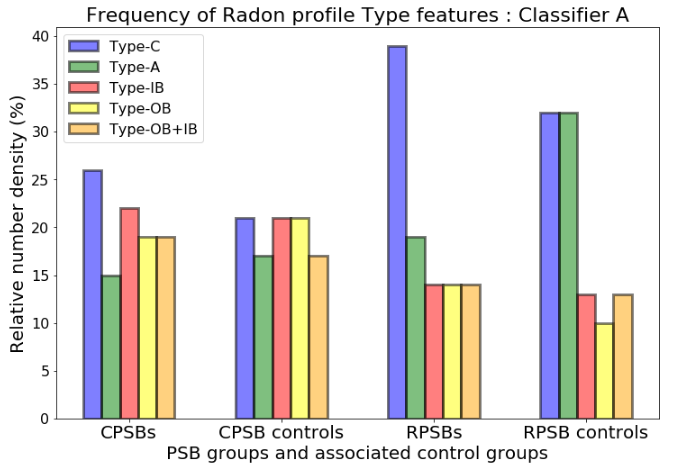
\includegraphics[width=\columnwidth]{images/JupyterPlots/PROFILE-GROUPS-CLASSIFIER-A.png}
    \caption[Radon profile Type classifications determined by classifier A]{The results of the Radon profile visual classification exercise obtained by classifier A is shown for the 4 galaxy groups of interest: CPSBs, CPSB controls, RPSBs and their controls. The numerical frequency of each of the 5 Radon profile type features from Table \ref{tab:Radon-VC-results} are displayed in this grouped bar plot. The colour coding of each type feature is shown in the legend.}
    \label{fig:Radon-grouped-barchart}
\end{figure}

\begin{table}
\centering
\caption{CPSBs with PA offset \textgreater 30\textdegree\ matched with their visually determined Radon profile Type.}
\label{tab:offsetCPSBs-Radon-Type}
\begin{tabular}{lcccc}
\hline
PlateIFU  & Stellar PA & H$\alpha$ PA & $\Delta$PA & Radon profile\\
  & (deg.) & (deg.) & (deg.) & Type \\
\hline
8313-6101 & 5 & 307 & 58 & OB \\
8655-1902 & 335 & 127 & 152 & OB+IB \\
8725-1902 & 22 & 175 & 153 & OB+IB \\
8938-6102 & 214 & 47.5 & 166.5 & C \\
9494-3701 & 140.5 & 243 & 102.5 & C \\
\hline
\end{tabular}
\end{table}

\begin{table}
\centering
\caption[RPSBs with PA offset \textgreater 30\textdegree\ matched with their visually determined Radon profile Type]{Similar to Table \ref{tab:offsetCPSBs-Radon-Type}. RPSBs with PA offset \textgreater 30\textdegree\ matched with their visually determined Radon profile Type.}
\label{tab:offsetRPSBs-Radon-Type}
\begin{tabular}{lcccc}
\hline
PlateIFU   & Stellar PA & H$\alpha$ PA & $\Delta$PA & Radon profile \\
  & (deg.) & (deg.) & (deg.) & Type\\
\hline
8080-3704 & 24 & 154 & 130 & C \\
8262-3701 & 153.5 & 118.5 & 35 & C \\
8323-6103 & 109.5 & 313.5 & 156 & C \\
8439-6104 & 5.5 & 107 & 101.5 & A \\
8453-3704 & 44 & 91 & 47 & C \\
8486-1901 & 295.5 & 85 & 149.5 & C \\
8554-3701 & 250 & 68 & 178 & OB \\
8932-12704 & 166.5 & 134.5 & 32 & A \\
9872-3701 & 208.5 & 81 & 127.5 & OB+IB \\
\hline
\end{tabular}
\end{table}

It is noted the majority of PSBs with $\Delta$PA offsets \textgreater 30\textdegree\ listed in Tables \ref{tab:offsetCPSBs-Radon-Type} and \ref{tab:offsetRPSBs-Radon-Type} show constant or asymmetric radial Radon profiles, however a few outer and inner bend profiles are evident. 

% \subsection{Independent visual classification}
\label{independent-classification}
An independent Radon profile classification exercise was carried out by a second classifier, Classifier B, following the same procedure as described in Section \ref{sec:Radon-classification}. The results of this supplementary classification are summarised in Table \ref{tab:Radon-VC2-results}, and displayed graphically in Figure \ref{fig:Radon-grouped-barchart-B}. The results obtained by Classifier B can be compared with and contrasted to the results obtained by Classifier A, as presented earlier in Table \ref{tab:Radon-VC-results} and Figure \ref{fig:Radon-grouped-barchart}.

\begin{table*}
\caption[Radon profile visual classification CPSB and RPSB samples and their control galaxies - classifier B]{Results of the supplementary Radon profile visual classification assessments for CPSB and RPSB samples and their control galaxies. The information presented is as per Table  \ref{tab:Radon-VC-results} but provides the profile classification results visually assessed by independent classifier B.}
\label{tab:Radon-VC2-results}
\begin{tabular}{lccccccc}
\hline
 & \begin{tabular}[c]{@{}c@{}}Classified \end{tabular} & Constant & Inner Bend & Outer Bend & \begin{tabular}[c]{@{}c@{}}Inner Bend + \\ Outer Bend\end{tabular} & Asymmetric & \begin{tabular}[c]{@{}c@{}}Not\\ Classified\end{tabular} \\
Galaxy group &  & (Type-C) & (Type-IB) & (Type-OB) & (Type-IB+OB) & (Type-A) & (NC) \\
 \hline
CPSBs & 28 & 1 (4\%) & 4 (14\%) & 5 (18\%) & 5 (18\%) & 13 (46\%) & - \\
CPSB controls & 29 & 2 (7\%) & 3 (10\%) & 1 (3\%) & 5 (17\%) & 18 (62\%) & 1 \\
RPSBs & 36 & 1 (3\%) & 6 (17\%) & 7 (19\%) & 5 (14\%) & 17 (47\%) & - \\
RPSB controls & 34 & 0 (0\%) & 4 (11\%) & 4 (11\%) & 7 (19\%) & 19 (53\%) & 2 \\
\hline
Totals & 127 & \multicolumn{1}{l}{ 4 (3\%)} & 17 (13\%) & 17 (13\%) & 22 (17\%) & 67 (53\%) & 3 \\
\hline
\end{tabular}
\end{table*}


\begin{figure}
    \centering
    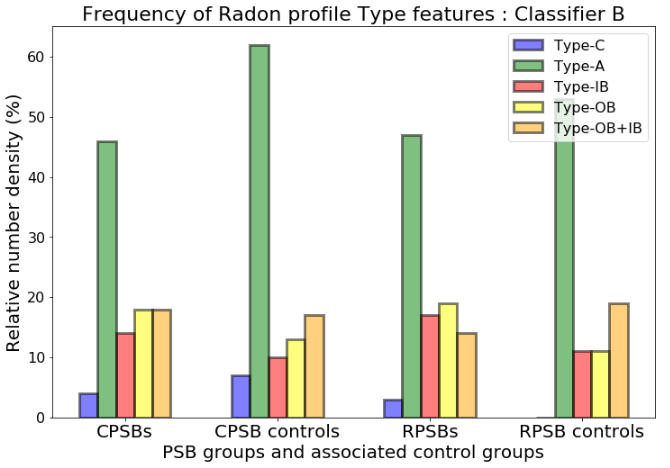
\includegraphics[width=\columnwidth]{images/JupyterPlots/PROFILE-TYPES-CLASSIFIER-B.png}
    \caption[Radon profile Type classifications determined by Classifier B]{The results of the Radon profile visual classification exercise obtained by Classifier B is shown for the 4 galaxy groups of interest: CPSBs, CPSB controls, RPSBs and their controls. The numerical frequency of each of the 5 Radon profile type features from Table \ref{tab:Radon-VC2-results} are presented graphically in this grouped bar plot. The colour coding of each type feature is shown in the legend.}
    \label{fig:Radon-grouped-barchart-B}
\end{figure}

We note a significant disparity in the the numbers classified in each of the Type categories as determined by Classifiers A and B. The disparity is particularly noticeable for the categorisation of Type-C (constant) and Type-A (asymmetric) profiles. This imbalance may be due to the similarity of the guideline examples given in Figure 7 of \cite{2018MNRAS.480.2217S}. Both the example profiles display some measure of asymmetry and also show a relatively constant profile in their central regions, around radius $\rho = 0$. In fact there is some indication of inner bend features in both the Type-C and Type-A examples. Evidently visual classification is difficult, and this comment was made by both classifiers. We continue further discussion on this point in Section \ref{sec:discussion}. Setting aside the difficulties of Type-A and Type-C classifications, we note that similar numbers galaxies with with bend-type features, Type-OB, Type-IB and Type-OB+IB were identified by both classifiers. We emphasise, however, that there was still considerable variation in classification for specific individual galaxies. The results of the two independent classifications (Classifiers A and B) for the 3 bend-feature categories, in each of the 4 galaxy groups, are summarised in Table \ref{tab:Radon-VC3-results}. There is little to infer from these results, maybe only that both classifiers determined similar numbers of Types in each galaxy category. This similarity is strongly contradicted, however, by the classifications determined by Classifiers A and B for specific galaxies. This can be seen by comparing the Type classification listings of Tables \ref{tab:full-visual-classification} and \ref{tab:visual-classification-B} in Appendix \ref{sec:visual-classification-tables}.

\begin{table*}
\caption[Comparison of Radon profile classifications by classifiers A and B, excluding Types A and B]{Comparison of Radon profile Type classifications provided by Classifiers A and B, excluding Type-C and Type-A profiles.}
\label{tab:Radon-VC3-results}
\begin{tabular}{lccccccccc}
\hline
 & \multicolumn{3}{c}{Classifier A} & \multicolumn{3}{c}{Classifier B} \\ 
Group & Type-IB & Type-OB & Type-IB+OB & \multicolumn{1}{l}{Type-IB} & \multicolumn{1}{l}{Type-OB} & \multicolumn{1}{l}{Type-IB+OB} \\
\hline
CPSBs & 6 & 5 & 5 & 4 & 5 & 5 \\
CPSB controls & 7 & 6 & 5 & 3 & 1 & 5 \\
RPSBs & 5 & 5 & 5 & 6 & 7 & 5 \\
RPSB controls & 4 & 3 & 4 & 4 & 4 & 7 \\
\hline
Totals & 22 & 19 & 19 & 17 & 17 & 22 \\
\hline
\end{tabular}
\end{table*}


\section{Discussion and conclusions}
\label{sec:discussion}
We have four topics to discuss here:
\begin{itemize}
\item \textbf{Velocity map binning methods:} a technical discussion on the comparative merits of alternative MaNGA velocity map binning methods and IFU sizes to obtain best resolution Radon profile traces.
\item \textbf{The relationship between Radon profiles classes and morphology:} we discuss a possible correlation between Radon transform trace profile Types and galaxy morphology.
\item \textbf{Findings and conclusions:} a review of the significant findings of the project and presentation of our conclusions.
\item \textbf{Future work:} we present suggested topics for future work noted during the course of the project. 
\end{itemize}

\subsection{Velocity map binning methods}
\label{sec:binning-methods}
The MaNGA DAP utilises various spaxel binning models to process the IFU fibre bundle data into the output maps. The available binning schemes used to produce gas and stellar velocity maps, together with a brief description of each are listed below.

\begin{itemize}
    \item SPX - single spaxel measurements i.e. no binning.
    \item VOR10 - Voronoi binning, an adaptive spatial binning method where low signal-to-noise (S/N) ratio spaxels are grouped to achieve an overall S/N of 10  \citep{2003MNRAS.342..345C, 2019arXiv190100856W}.
    \item HYB10 - Hybrid binning: Voronoi S/N 10 binning for stellar velocity maps, but unbinned for emission line properties which are used to generate gas velocity maps.
\end{itemize}  

In this study we have utilised MaNGA datacubes released in DR15 MPL-7 which have been processed in the DAP using the hybrid HYB10 binning model, i.e. using VOR10 binning for the stellar velocity maps. However, the MaNGA project team currently have an internal dataset available, MPL-8. Datacubes in MPL-8 include VOR10 and SPX binning schema. We were interested to make a comparison of the Radon trace profiles generated from the datacubes using the Voronoi and SPX binning schemas. A limited sample of MPL-8 cubes were made available for this comparison exercise. We selected 2 galaxies from our samples with stellar velocity maps having poor spatial definition, and another 2 with good resolution in order to compare the Radon transform profiles using the Voronoi binning and SPX (unbinned) methods. The selected datacubes were firstly, examples of good resolution/definition in stellar velocity maps:

\begin{itemize}
    \item 7977-12704
    \item 8322-1901
\end{itemize}

and secondly, examples of poor resolution/definition in stellar velocity maps, i.e. having a blotchy appearance, due to spatial binning of low S/N spaxels, or with masked spaxels:

\begin{itemize}
    \item 9088-12703
    \item 8993-6104
\end{itemize}

The stellar velocity maps together with their Radon transform and trace profiles for these well defined example 7977-12704 are shown in Figure \ref{fig:binning-comparison}. The differences being the binning models of the input stellar velocity maps: Voronoi binning in the left-hand panel and SPX binning on the right. A comparison shows that there is little difference in the Radon transform and Radon profile plots. It is also apparent that the Radon transform algorithm for the SPX velocity maps yields a greater number of valid data points in the trace plot. We conclude that both VOR10 and SPX binned maps would lead to the same Type classification in these cases. This conclusion was also obtained for other galaxy showing good resolution in the stellar velocity map,  8322-1901 (figure not included). 

However, the same conclusion does not apply for the low resolution stellar velocity map examples, 8993-6104 shown in Figure \ref{fig:binning-comparison2} and 9088-12703 (figure not included). In these cases, at first sight, there are marked differences in the extent of spatial coverage and shapes of the velocity field PA, the Radon transform minimum and the Radon profile. In particular the control galaxy 8993-6104 displays a clearly asymmetric Radon profile with VOR10 binning, but could possibly be interpreted as an outer bend in the Radon profile trace of the SPX map. However, on closer inspection, looking at the  range the trace plots, the same bend feature at Radon transform coordinates [$\rho$, $\theta$]=[-6,+2],[20, 50] is apparent in both binning model plots. The asymmetric feature at $\rho$ \textgreater\ +2 apparent in the left Voronoi binned trace is not evident in the SPX output shown in the right-hand panel. Although these differences can be expected due to the exclusion of low S/N low spaxels in the SPX maps, crucially this can easily lead to a different visual classification result between the transforms of Voronoi binned and SPX velocity field maps. 
\begin{figure*}
    \centering
    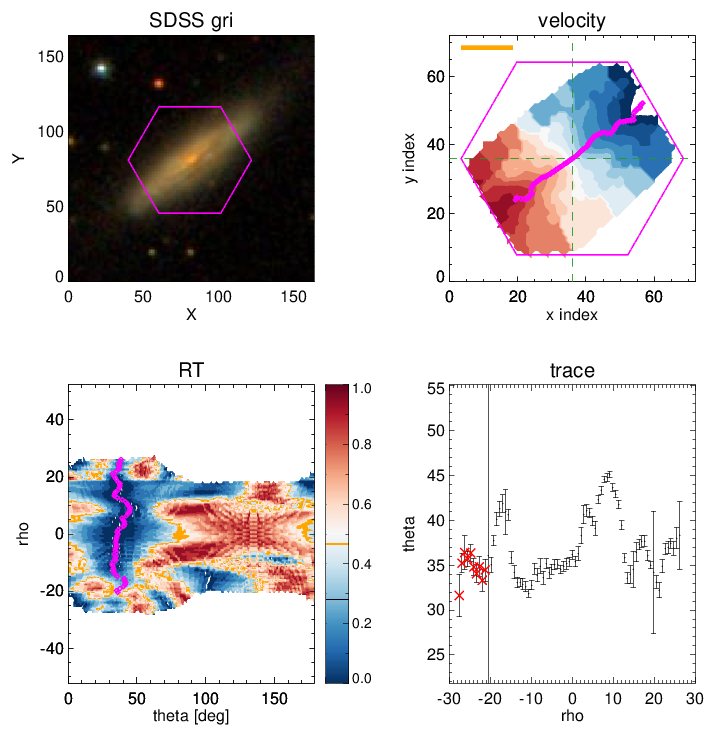
\includegraphics[width=\columnwidth]{images/RadonPlots/RT-SNIPS-NEW/7977-12704-VOR10-MILESHC-MILESHC-1-SNIP.png}
    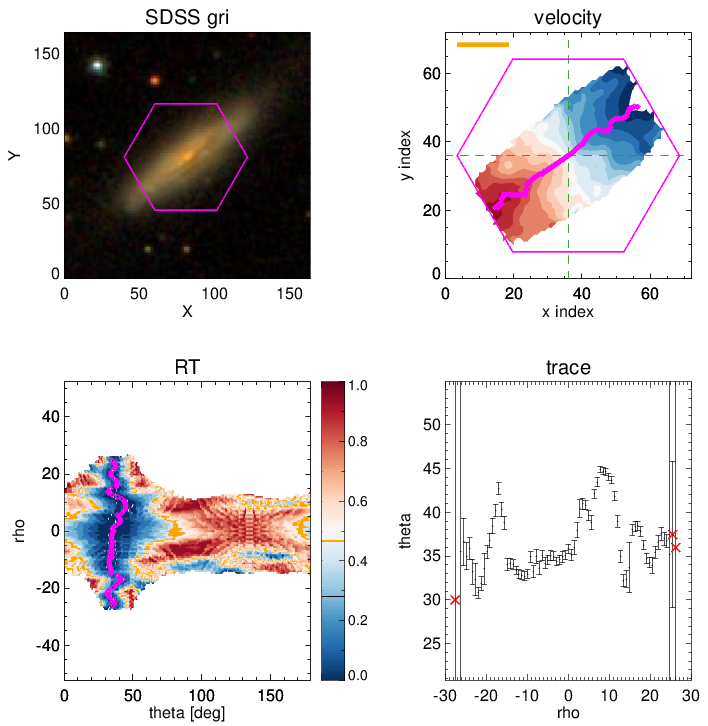
\includegraphics[width=\columnwidth]{images/RadonPlots/RT-SNIPS-NEW/7977-12704-SPX-MILESHC-MILESHC-1-SNIP.png}
    \caption[Comparison of velocity map binning schemes for a high resolution map]{Comparison of stellar velocity map binning methods using the Radon transform output graphic for the galaxy 7977-12704. The velocity map has good resolution using both schemes. In the left panel the transform RT and profile trace plots are generated from the stellar velocity map with Voronoi binning. The plots in the right panel were produced from the stellar velocity map using single spaxel SPX resolution. The layout of the 4 subplots in each panel is as described in Figure \ref{fig:8442-3704-complete}.}
    \label{fig:binning-comparison}
\end{figure*}

\begin{figure*}
    \centering
    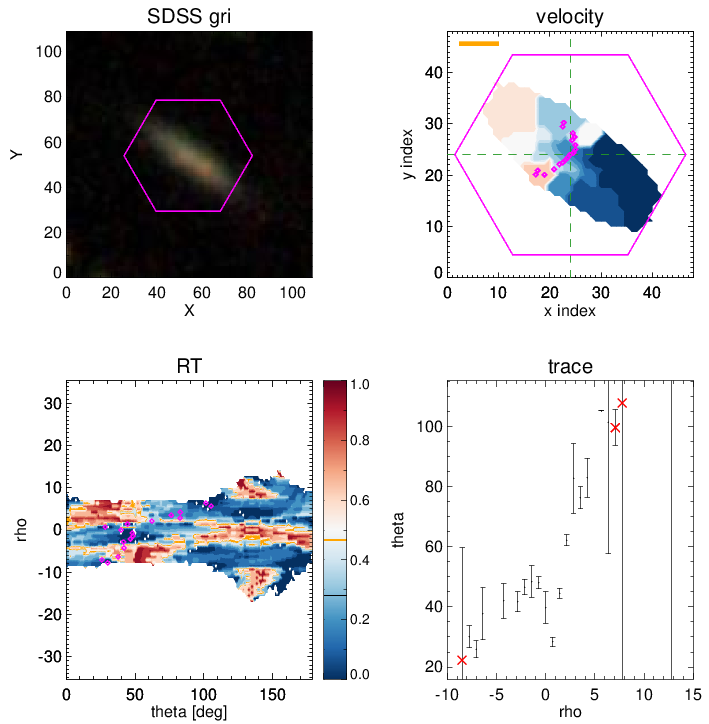
\includegraphics[width=\columnwidth]{images/RadonPlots/RT-SNIPS-NEW/8993-6104-VOR10-MILESHC-MILESHC-1-SNIP.png}
    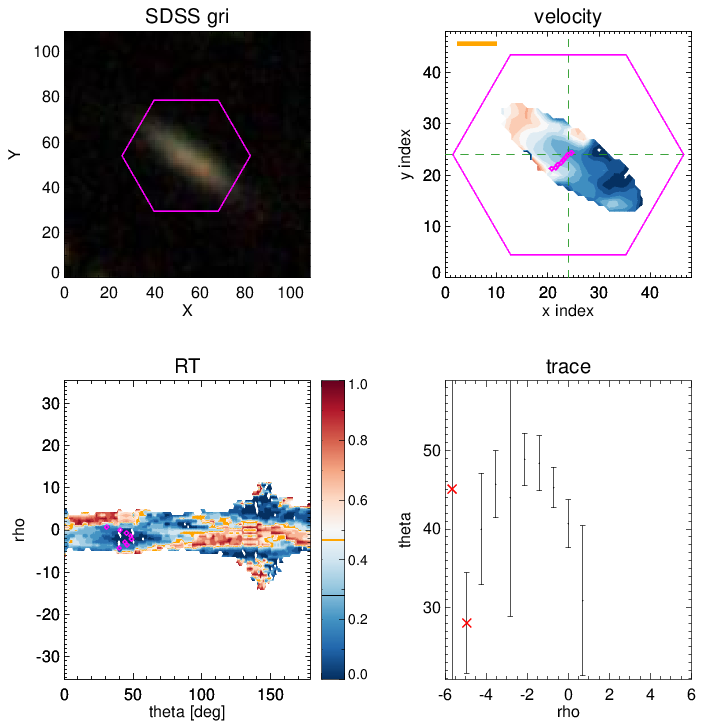
\includegraphics[width=\columnwidth]{images/RadonPlots/RT-SNIPS-NEW/8993-6104-SPX-MILESHC-MILESHC-1-SNIP.png}
    \caption[Comparison of velocity map binning schemes for a low resolution map]{Comparison of velocity map binning schemes for a low resolution map. Radon transform output graphic for the galaxy 8993-6104 with a low resolution stellar velocity map. In the left panel the transform RT and profile trace plots are generated from the stellar velocity map with Voronoi binning. The plots in the right panel were produced from the stellar velocity map using single spaxel SPX binning. The layout of the 4 subplots in each panel is as described in Figure \ref{fig:8442-3704-complete}.}
    \label{fig:binning-comparison2}
\end{figure*}




\subsection[Correlation between Radon profiles and morphology]{Correlation between Radon profile types and morphological features}
\label{correlations}
\cite{2018MNRAS.480.2217S} made a considerable effort to explore a possible correlation between the observed frequencies of the 5 Radon profile types (Type-C, Type-A, Type-IB, Type-OB and Type-OB+IB) and underlying morphological features determined from the Galaxy Zoo morphology classification project. They found some evidence of weak associations between Radon profile trace type and morphological features, as discussed in detail in their Section 5. These correlations are subjective and certainly not exclusive, and care must be taken to follow their arguments closely. The most prevalent of the identified relationships can be broadly interpreted as follows:
\begin{itemize}
    \item Type-C: Constant profile - frequently apparent in unbarred galaxies.
    \item Type-A: Asymmetric - can be associated with tidal interactions.
    \item Type-IB: Inner bends - prevalent in strongly barred galaxies.
    \item Type-OB: Outer bends - associated with kinematic warps.
\end{itemize}

\blue{Following this discussion the prevailing reasoning is that outer bend-type features, Type-OB, may be associated with kinematic warps and indicative of past mergers. Also Type-C (constant) profiles were expected to be associated with indicate uniform, undisturbed velocity fields. As reported in the results Section \ref{sec:comparison-of-results} we found that 5 out of 14 PSBs with large $\Delta$PA$_{k}$ offsets were assigned Radon profile trace classification of Type-OB. We emphasise, however, that this result was determined by Classifier A, and there is no consensus with either Classifier B or in the limited number of automatic classifications that were available for our galaxies. Setting this point aside there may be some correlation between Radon profile Type-OB, large $\Delta$PA$_{k}$ and past major mergers driving quenching in post-starburst galaxies.}

\subsection{Findings}
\label{findings}

%TC:ignore
\green{Include a bit linking high S\'ersic index (CPSBs), high DeltaPAs (CPSBs), the K-S test, spheroidal morphology and CPSBs. How do we do that?}
%TC:endignore

Generally CPSBs show a wide range of kinematic position angle differences $\Delta$PA$_{k}$ \textgreater 30\textdegree\ with many in the range 90 \textless\ $\Delta$PA$_{k}$ \textless\ 180\textdegree. RPSBs show a smaller range in $\Delta$PA$_{k}$ with only a few over 90\textdegree. The majority of control galaxies have small kinematic position angle differences, mainly less than 25\textdegree. Significant misalignment in the gas and stellar velocity fields of CPSBs, and to a lesser extent RPSBs, is indicative of past or ongoing disturbances as could be expected from major mergers.
We note that the distribution $\Delta$PA$_{k}$ is markedly different when comparing CPSBs with CPSB controls. This trait is also present, but to a lesser extent, in the comparison of the RPSB $\Delta$PA$_{k}$ with their controls. The distribution in differential kinematic position angles is similar for both control groups. These observations are supported by the results of K-S analysis in Section \ref{sec:K-S-test} where we find the difference in $\Delta$PA$_{k}$ of both PSB groups compared to their control groups to be statistically significant. \green{From this we conclude that there is evidence presented from the $\Delta$PA$_{k}$ distributions, the K-S statistical analysis performed on these $\Delta$PA$_{k}$ distributions, together with the distributions in S\'ersic index that there is a evolutionary sequence from the normal (control) galaxies, to the disc-like RPSBs and on to the redder spheroidal CPSBs. The quenching of star formation in ring-shaped features in RPSBs and the central regions of CPSBs provides compelling evidence of past major mergers, triggering morphological transformation from late-type galaxies to spheroids and an evolutionary transition from the blue cloud, through the green valley, and on towards the red sequence.}

We compared the Radon profile trace results obtained from stellar velocity maps employing Voronoi VOR10 binning versus the single spaxel SPX unbinned schema. We obtained cleaner trace profiles (i.e. easier to classify) with a greater number of valid data points and tighter error bars from high S/N maps based on single spaxel SPX binning. For future studies, given a large enough sample of PSBs, we should avoid Voronoi binned maps where possible and use SPX maps a cut of S/N \textgreater say 3-5 in single spaxels.

Kinematic PA analysis versus Radon transform: as described in Section \ref{sec:motivation} the Radon transform provides distinct advantages over the kinematic $\Delta$PA$_{k}$  method. Radon transforms provide a detailed trace of position angle across the velocity field enabling local regions of radial variation to be identified. Kinematic PAs require both stellar and gas velocity fields to be mapped but post-starburst galaxies may possess little gas. The Radon transform can trace disturbances as evidence of mergers using the stellar velocity field alone.

Kinematic warps in the stellar discs of early-type field galaxies can be attributed to multiple stellar components suggestive of past dry mergers \citep{2005AJ....130.2647V}, although warps can also be sustained by tidal interactions.
From this we draw the simple conclusion that Radon trace profiles displaying outer bends, Type-OB or Type-OB+IB can be considered prospective candidates past major mergers, or post-mergers. From Table \ref{tab:Radon-VC-results} we find that 10 of of 27 CPSBs (37\%) reveal Type-OB or Type-OB+IB Radon profile signatures. As an area for future study we should consider a similar exercise to utilise the Galaxy Zoo morphology classifications together with Radon profile feature types as identified in this present study. 

Visual classification of Radon profile types was found to be very difficult, our classifiers agreed on this point. In addition our classifiers arrived at varying interpretations of profile type class for most of the galaxies. Although the same written classification procedure was followed, the method was quite loosely defined, recognising the difficulties in relating the race plots to the examples. With so few classifiers involved we conclude that there is significant classification error present in our results, remembering the the Galaxy Zoo project engaged $\sim10^5$ classifiers to minimise classification error.

The results of the visual classification of the 5 Radon trace type profiles for CPSBs, RPSBs and their control groups as presented in Table \ref{tab:Radon-VC-results} and shown graphically in Figure \ref{fig:Radon-grouped-barchart} are quantitatively similar in number. This was unexpected and is presently not fully explained. We can, however, expect more galaxies with constant features in the RPSB groups than the CPSBs as RPSBs exhibit PSB features in local regions only while we can expect a higher percentage of the non-linear features, i.e. inner and outer bends and composite bend features Type-OB+IB, to be apparent in the trace profiles of CPSBs due to their central and more widespread post-starburst regions. Incorporating the the results from the second classifier a picture emerges that Type-OB features are 70\% more prevalent in both the CPSB sample to controls, and RPSBs to their controls. 

\subsection{Summary}
\label{summary}
In the past major mergers have been detected using imaging techniques. In this project we have attempted to identify past major mergers in PSB galaxies, firstly by investigating the distributions of differences in stellar and gas velocity field kinematic position angles, and secondly by using the Radon transform method to reveal radial variation in kinematic position angles. This has not proved conclusive. More work is required on the classification of kinematic features apparent in the Radon profile trace plots. However, \cite{2019DDA....5020304N} have recently announced work on a method which promises to increase the accuracy of merger detection using a method that integrates imaging and kinematic analysis techniques. This extended method will combine SDSS imaging (providing morphological observations) with MaNGA  kinematic maps, towards enhanced identification of merger and post-merger signatures. When available, this technique should be applied to our PSB and control samples to detect evidence of past mergers. With this technique we may be able to increase our likelihood estimates of positive detection of past major merger events in post-starburst galaxies.



\section*{Acknowledgements}

The Acknowledgements section is not numbered. Here you can thank helpful
colleagues, acknowledge funding agencies, telescopes and facilities used etc.
Try to keep it short.

%%%%%%%%%%%%%%%%%%%%%%%%%%%%%%%%%%%%%%%%%%%%%%%%%%

%%%%%%%%%%%%%%%%%%%% REFERENCES %%%%%%%%%%%%%%%%%%

% The best way to enter references is to use BibTeX:

%\bibliographystyle{mnras}
%\bibliography{example} % if your bibtex file is called example.bib
%----------- REFERENCES ------------------%
\bibliographystyle{mnras}
\bibliography{JPbib2019} 


%%%%%%%%%%%%%%%%%%%%%%%%%%%%%%%%%%%%%%%%%%%%%%%%%%

%%%%%%%%%%%%%%%%% APPENDICES %%%%%%%%%%%%%%%%%%%%%

% include your \appendix here

\appendix
\onecolumn

\section{Visual classification of Radon profiles}
\label{sec:visual-classification-tables}

%TC:ignore

Here are the results of the Radon profile visual assessment for the PSB galaxy targets and their controls. The Radon profile class is determined from the relative Radon profile feature strengths: C, IB, OB, OB+IB and A. The classification methodology is described in Section \ref{sec:Radon-classification}.

% Please add the following required packages to your document preamble:
% \usepackage{longtable}
% Note: It may be necessary to compile the document several times to get a multi-page table to line up properly

\begin{longtable}{p{2.1cm}p{0.8cm}p{0.8cm}p{0.8cm}p{0.8cm}p{0.8cm}p{1.5cm}p{1.5cm}p{1.2cm}}
\caption{Complete Radon profile visual classification determination for 127 galaxies in the target sample of PSBs and control galaxies.}
\label{tab:full-visual-classification} \\

\hline
\\
PLATEIFU & C & IB & OB & OB+IB & A & Primary & Secondary & Final \\
\\
\hline
\\
\endfirsthead
%
{{\bfseries \tablename\ \thetable{} -- cont.}}
\\
\hline
\\
PLATEIFU & C & IB & OB & OB+IB & A & Primary & Secondary & Final \\
\\
\hline
\\
\endhead

\\
\hline 
{{More ...}}
\endfoot
\hline
\endlastfoot

7958-1901 & 2 & 0 & 0 & 0 & 2 & A & C+A & A \\
7964-1902 & 2 & 0 & 0 & 0 & 0 & C & C & C \\
7977-12703 & 2 & 1 & 0 & 1 & 0 & C & C+IB & C \\
7977-12704 & 1 & 1 & 1 & 2 & 1 & OB+IB & IB & A \\
8077-6102 & 1 & 1 & 1 & 2 & 0 & OB+IB & OB+IB & OB+IB \\
8080-3702 & 2 & 2 & 0 & 2 & 1 & C & C+IB & C \\
8080-3704 & 2 & 1 & 0 & 1 & 0 & C & C+IB & C \\
8081-3702 & 0 & 0 & 0 & 0 & 2 & A & A & A \\
8082-3704 & 0 & 1 & 2 & 3 & 0 & OB+IB & OB & OB+IB \\
8083-12703 & 0 & 2 & 1 & 3 & 0 & IB & OB & IB \\
8084-6103 & 1 & 2 & 0 & 2 & 1 & IB & C+IB & A \\
8084-9101 & - & - & - & - & - & NC & NC & NC \\
8085-6104 & 0 & 2 & 2 & 4 & 0 & OB+IB & OB+IB & OB+IB \\
8139-12701 & 0 & 1 & 0 & 1 & 2 & A & A+IB & A \\
8143-3703 & 2 & 1 & 0 & 1 & 0 & C & C+IB & C \\
8146-1901 & 0 & 1 & 0 & 1 & 2 & A & A & A \\
8243-12704 & 2 & 0 & 1 & 1 & 0 & C & C+OB & C \\
8249-3704 & 1 & 2 & 2 & 4 & 1 & OB+IB & OB+IB & OB \\
8250-6101 & 2 & 2 & 0 & 2 & 1 & C & C+IB & C \\
8250-6104 & 2 & 1 & 0 & 1 & 0 & C & C+IB & C \\
8255-3703 & 0 & 2 & 0 & 2 & 2 & IB & A+IB & IB \\
8259-12702 & 2 & 0 & 0 & 0 & 0 & C & C & C \\
8261-6103 & 2 & 0 & 0 & 0 & 0 & C & C & C \\
8262-3701 & 2 & 1 & 0 & 1 & 0 & C & C+IB & C \\
8262-3703 & 2 & 0 & 2 & 2 & 0 & OB & OB & OB \\
8262-12701 & 1 & 2 & 0 & 2 & 0 & IB & C+IB & IB \\
8274-12701 & 1 & 2 & 2 & 4 & 0 & OB+IB & OB+IB & C \\
8313-6101 & 1 & 1 & 2 & 3 & 0 & OB & OB & OB \\
8315-3703 & 0 & 2 & 0 & 2 & 2 & IB & A+IB & IB \\
8322-1901 & 2 & 0 & 0 & 0 & 0 & C & C & C \\
8323-6103 & 2 & 1 & 0 & 1 & 0 & C & C+IB & C \\
8331-6104 & 0 & 2 & 1 & 3 & 1 & OB+IB & IB & OB+IB \\
8335-12704 & 1 & 2 & 0 & 2 & 0 & IB & IB & IB \\
8439-6104 & 0 & 1 & 2 & 3 & 2 & A & A+OB & A \\
8440-1901 & 1 & 0 & 0 & 0 & 2 & A & A & A \\
8440-6104 & 0 & 1 & 2 & 3 & 0 & OB & OB+IB & OB \\
8440-12701 & 2 & 0 & 0 & 0 & 0 & C & C & C \\
8442-3704 & 1 & 0 & 2 & 2 & 0 & OB & C & OB \\
8453-3704 & 2 & 1 & 0 & 1 & 0 & C & C & C \\
8458-6102 & 0 & 1 & 0 & 1 & 2 & A & A+IB & A \\
8461-9102 & 0 & 1 & 2 & 3 & 1 & OB & OB+IB & OB+IB \\
8466-12702 & 2 & 0 & 0 & 0 & 0 & C & C & C \\
8486-9101 & 1 & 2 & 2 & 4 & 0 & OB+IB & IB & C \\
8547-9102 & 1 & 0 & 0 & 0 & 1 & C & A & C \\
8550-12704 & 1 & 1 & 2 & 3 & 0 & OB+IB & OB+IB & C \\
8553-12701 & 0 & 1 & 1 & 2 & 0 & NC & NC & NC \\
8554-3701 & 0 & 1 & 2 & 3 & 1 & OB & A & OB \\
8555-1901 & 2 & 0 & 0 & 0 & 0 & C & A & C \\
8555-3701 & 0 & 2 & 0 & 2 & 1 & IB & A+IB & IB \\
8592-6101 & 0 & 2 & 0 & 2 & 2 & A & A+IB & A \\
8597-12701 & 1 & 0 & 2 & 2 & 1 & OB & OB & OB \\
8602-6101 & 0 & 2 & 0 & 2 & 0 & IB & IB & IB \\
8604-3702 & 0 & 0 & 2 & 2 & 0 & OB & OB & OB \\
8612-9102 & 0 & 1 & 0 & 1 & 1 & A & A+IB & IB \\
8623-3702 & 1 & 2 & 0 & 2 & 0 & IB & IB & IB \\
8623-9102 & 0 & 1 & 2 & 3 & 1 & OB+IB & OB+IB & OB \\
8624-6103 & 0 & 2 & 0 & 2 & 1 & IB & A+IB & IB \\
8624-12704 & 1 & 0 & 2 & 2 & 0 & OB & OB & OB \\
8625-3703 & 2 & 0 & 0 & 0 & 0 & C & C & C \\
8625-9102 & 0 & 1 & 1 & 2 & 2 & A & OB+IB & A \\
8655-1902 & 2 & 1 & 0 & 1 & 1 & C & OB+IB & OB+IB \\
8655-3701 & 0 & 1 & 2 & 3 & 0 & OB+IB & OB & OB+IB \\
8713-3701 & 1 & 2 & 0 & 2 & 0 & IB & IB & IB \\
8716-12704 & 0 & 2 & 2 & 4 & 0 & OB+IB & IB & OB+IB \\
8718-6101 & 0 & 2 & 0 & 2 & 2 & A & A+IB & IB \\
8718-9102 & 0 & 0 & 0 & 0 & 0 & NC & NC & NC \\
8724-6103 & 0 & 2 & 2 & 4 & 0 & OB+IB & OB+IB & OB+IB \\
8725-1902 & 0 & 2 & 1 & 3 & 0 & IB & IB & OB+IB \\
8726-12702 & 0 & 0 & 1 & 1 & 2 & A & A & A \\
8727-12704 & 0 & 2 & 0 & 2 & 1 & IB & IB & IB \\
8932-1901 & 1 & 2 & 0 & 2 & 0 & IB & IB & OB+IB \\
8932-6103 & 2 & - & 0 & - & 0 & C & C & C \\
8932-12704 & 0 & 1 & 0 & 1 & 2 & A & A+IB & A \\
8933-3704 & 0 & 1 & 0 & 1 & 2 & A & A+IB & A \\
8934-9101 & 0 & 0 & 0 & 0 & 2 & A & A & NC \\
8935-12701 & 1 & 2 & 0 & 2 & 0 & IB & IB & IB \\
8938-6102 & 1 & 0 & 1 & 1 & 0 & C & C & C \\
8939-3701 & 1 & 2 & 2 & 4 & 0 & OB+IB & OB+IB & OB+IB \\
8940-3703 & 2 & 0 & 0 & 0 & 0 & C & C & C \\
8940-6101 & 1 & 0 & 2 & 2 & 0 & OB & OB & OB \\
8941-3701 & 2 & 0 & 0 & 0 & 0 & C & C & C \\
8943-1901 & 2 & 1 & 0 & 1 & 0 & C & IB & IB \\
8944-1902 & 0 & 0 & 1 & 1 & 2 & A & A+OB & OB \\
8945-12703 & 2 & 1 & 1 & 2 & 0 & C & OB+IB & C \\
8950-3704 & 1 & 2 & 2 & 4 & 0 & OB+IB & OB+IB & OB+IB \\
8950-6101 & 0 & 0 & 0 & 0 & 2 & A & A & A \\
8950-12705 & 2 & 0 & 0 & 0 & 0 & C & C & C \\
8979-1902 & 0 & 0 & 2 & 2 & 0 & OB & OB & OB \\
8979-12701 & 1 & 2 & 2 & 4 & 0 & OB+IB & OB+IB & OB+IB \\
8982-6104 & 1 & 2 & 0 & 2 & 0 & IB & IB & IB \\
8987-9102 & 1 & 1 & 2 & 3 & 0 & OB & OB+IB & OB \\
8990-12701 & 0 & 0 & 0 & 0 & 2 & A & A & A \\
8992-1902 & 0 & 0 & 2 & 2 & 0 & OB & OB & OB \\
8992-6103 & 2 & 0 & 0 & 0 & 0 & C & C & C \\
8993-6104 & 0 & 0 & 0 & 0 & 2 & A & A & A \\
8995-9101 & 2 & 0 & 0 & 0 & 0 & C & C & C \\
8996-3704 & 0 & 0 & 0 & 0 & 2 & A & A & A \\
8997-3703 & 1 & 1 & 2 & 3 & 0 & OB & OB & OB \\
8997-3704 & 2 & 0 & 0 & 0 & 0 & C & C & C \\
9029-6103 & 2 & 0 & 0 & 0 & 0 & C & C & C \\
9031-12701 & 1 & 1 & 0 & 1 & 0 & C & IB & IB \\
9043-6104 & 1 & 0 & 0 & 0 & 2 & A & C & A \\
9047-3701 & 1 & 0 & 0 & 0 & 2 & A & A & A \\
9047-12702 & 0 & 0 & 0 & 0 & 2 & A & A & A \\
9048-6101 & 0 & 0 & 0 & 0 & 2 & A & A & A \\
9085-1902 & 0 & 1 & 0 & 1 & 1 & IB & A+IB & IB \\
9088-12703 & - & - & - & - & - & NC & NC & NC \\
9181-12705 & 0 & 2 & 0 & 2 & 1 & IB & A+IB & OB \\
9184-1901 & 0 & 2 & 0 & 2 & 1 & IB & A+IB & IB \\
9184-3703 & 0 & 1 & 0 & 1 & 2 & A & A+IB & A \\
9194-3702 & 1 & 0 & 0 & 0 & 2 & A & A & C \\
9487-9102 & 1 & 2 & 2 & 4 & 0 & OB+IB & OB+IB & OB+IB \\
9493-12705 & 2 & 1 & 1 & 2 & 1 & C & C & IB \\
9494-3701 & 2 & 0 & 0 & 0 & 0 & C & C & C \\
9494-3703 & 2 & 1 & 0 & 1 & 0 & C & C & C \\
9502-1901 & - & - & - & - & - & NC & NC & NC \\
9505-6102 & 2 & 1 & 0 & 1 & 0 & C & C & C \\
9505-6104 & 0 & 0 & 0 & 0 & 2 & A & A & A \\
9505-12701 & 2 & 1 & 0 & 1 & 0 & C & IB & IB \\
9509-9101 & 2 & 0 & 0 & 0 & 0 & C & C & C \\
9868-3702 & 1 & 2 & 2 & 4 & 0 & OB+IB & OB+IB & OB+IB \\
9870-12701 & - & - & - & - & - & NC & NC & NC \\
9871-1901 & - & - & - & - & - & NC & NC & NC \\
9871-3702 & 2 & 0 & 0 & 0 & 0 & C & C & C \\
9872-3701 & 1 & 2 & 2 & 4 & 0 & OB+IB & OB+IB & OB+IB \\
9876-3701 & 0 & 0 & 0 & 0 & 2 & A & A & A \\
9891-6102 & 0 & 1 & 0 & 1 & 2 & A & A+IB & IB \\
 &  &  &  &  &  &  &  &  \\
 &  &  &  &  &  &  &  & 
\end{longtable}
%TC:endignore


%%%%%%%%%%%%%%%%%%%%%%%%%%%%%%%%%%%%%%%%%%%%%%%%%%


% Don't change these lines
\bsp	% typesetting comment
\label{lastpage}
\end{document}

% End of mnras_template.tex